%% LyX 2.3.7 created this file.  For more info, see http://www.lyx.org/.
%% Do not edit unless you really know what you are doing.
\documentclass[journal,article,submit,pdftex,moreauthors]{Definitions/mdpi}
\usepackage[T1]{fontenc}
\usepackage[utf8]{inputenc}
\setcounter{secnumdepth}{1}
\setcounter{tocdepth}{1}
\usepackage{float}
\usepackage{url}
\usepackage{graphicx}

\makeatletter

%%%%%%%%%%%%%%%%%%%%%%%%%%%%%% LyX specific LaTeX commands.

\Title{An Innovative Hybrid Approach to Global Optimization}

\TitleCitation{An Innovative Hybrid Approach to Global Optimization}

\Author{Vasileios Charilogis$^{1}$,Glykeria Kyrou$^{2}$, Ioannis G. Tsoulos$^{3,*}$,
Anna Maria Gianni$^{4}$}

\AuthorNames{V. Charilogis, Glykeria Kyrou, I.G. Tsoulos, A.M. Gianni}

\AuthorCitation{Charilogis V.; Kyrou, G.;Tsoulos I.G.; Gianni A.M; }


\address{$^{1}$\quad{}Department of Informatics and Telecommunications,
University of Ioannina, Greece; v.charilog@uoi.gr\\
$^{2}$\quad{}Department of Informatics and Telecommunications, University
of Ioannina, Greece; g.kyrou@uoi.gr\\
$^{3}$\quad{}Department of Informatics and Telecommunications, University
of Ioannina, Greece; itsoulos@uoi.gr\\
$^{4}$\quad{}Department of Informatics and Telecommunications, University
of Ioannina, Greece; am.gianni@uoi.gr}


\corres{Correspondence: itsoulos@uoi.gr;}


\abstract{Global optimization is critical in engineering, computer science,
and various industrial applications, as it aims to find optimal solutions
for complex problems. The development of efficient algorithms has
emerged from the need for optimization, with each algorithm offering
specific advantages and disadvantages. An effective approach to solving
complex problems is the hybrid method, which combines established
global optimization algorithms. \textbf{This paper presents a hybrid
global optimization method, which produces trial solutions for an
objective problem, utilizing Genetic Algorithm genetic operators,
as well as solutions obtained through a linear search process. Then,
the generated solutions are used to form new test solutions, by applying
Differential Evolution techniques.} These operations are based on
samples derived either from internal line searches or genetically
modified samples in specific subsets of Euclidean space. Additionally,
other relevant approaches are explored to enhance the method's efficiency.
The new method was applied on a wide series of benchmark problems
from the recent literature and comparison was made against other established
methods of Global Optimization. }


\keyword{Optimization; Differential evolution; Genetic algorithm; Line search;
Evolutionary techniques; Stochastic methods; Hybrid methods.}

\newcommand*\LyXZeroWidthSpace{\hspace{0pt}}
%% Because html converters don't know tabularnewline
\providecommand{\tabularnewline}{\\}

%%%%%%%%%%%%%%%%%%%%%%%%%%%%%% User specified LaTeX commands.
%  LaTeX support: latex@mdpi.com 
%  For support, please attach all files needed for compiling as well as the log file, and specify your operating system, LaTeX version, and LaTeX editor.

%=================================================================


% For posting an early version of this manuscript as a preprint, you may use "preprints" as the journal and change "submit" to "accept". The document class line would be, e.g., \documentclass[preprints,article,accept,moreauthors,pdftex]{mdpi}. This is especially recommended for submission to arXiv, where line numbers should be removed before posting. For preprints.org, the editorial staff will make this change immediately prior to posting.

%--------------------
% Class Options:
%--------------------
%----------
% journal
%----------
% Choose between the following MDPI journals:
% acoustics, actuators, addictions, admsci, adolescents, aerospace, agriculture, agriengineering, agronomy, ai, algorithms, allergies, alloys, analytica, animals, antibiotics, antibodies, antioxidants, applbiosci, appliedchem, appliedmath, applmech, applmicrobiol, applnano, applsci, aquacj, architecture, arts, asc, asi, astronomy, atmosphere, atoms, audiolres, automation, axioms, bacteria, batteries, bdcc, behavsci, beverages, biochem, bioengineering, biologics, biology, biomass, biomechanics, biomed, biomedicines, biomedinformatics, biomimetics, biomolecules, biophysica, biosensors, biotech, birds, bloods, blsf, brainsci, breath, buildings, businesses, cancers, carbon, cardiogenetics, catalysts, cells, ceramics, challenges, chemengineering, chemistry, chemosensors, chemproc, children, chips, cimb, civileng, cleantechnol, climate, clinpract, clockssleep, cmd, coasts, coatings, colloids, colorants, commodities, compounds, computation, computers, condensedmatter, conservation, constrmater, cosmetics, covid, crops, cryptography, crystals, csmf, ctn, curroncol, currophthalmol, cyber, dairy, data, dentistry, dermato, dermatopathology, designs, diabetology, diagnostics, dietetics, digital, disabilities, diseases, diversity, dna, drones, dynamics, earth, ebj, ecologies, econometrics, economies, education, ejihpe, electricity, electrochem, electronicmat, electronics, encyclopedia, endocrines, energies, eng, engproc, ent, entomology, entropy, environments, environsciproc, epidemiologia, epigenomes, est, fermentation, fibers, fintech, fire, fishes, fluids, foods, forecasting, forensicsci, forests, foundations, fractalfract, fuels, futureinternet, futureparasites, futurepharmacol, futurephys, futuretransp, galaxies, games, gases, gastroent, gastrointestdisord, gels, genealogy, genes, geographies, geohazards, geomatics, geosciences, geotechnics, geriatrics, hazardousmatters, healthcare, hearts, hemato, heritage, highthroughput, histories, horticulturae, humanities, humans, hydrobiology, hydrogen, hydrology, hygiene, idr, ijerph, ijfs, ijgi, ijms, ijns, ijtm, ijtpp, immuno, informatics, information, infrastructures, inorganics, insects, instruments, inventions, iot, j, jal, jcdd, jcm, jcp, jcs, jdb, jeta, jfb, jfmk, jimaging, jintelligence, jlpea, jmmp, jmp, jmse, jne, jnt, jof, joitmc, jor, journalmedia, jox, jpm, jrfm, jsan, jtaer, jzbg, kidney, kidneydial, knowledge, land, languages, laws, life, liquids, literature, livers, logics, logistics, lubricants, lymphatics, machines, macromol, magnetism, magnetochemistry, make, marinedrugs, materials, materproc, mathematics, mca, measurements, medicina, medicines, medsci, membranes, merits, metabolites, metals, meteorology, methane, metrology, micro, microarrays, microbiolres, micromachines, microorganisms, microplastics, minerals, mining, modelling, molbank, molecules, mps, msf, mti, muscles, nanoenergyadv, nanomanufacturing, nanomaterials, ncrna, network, neuroglia, neurolint, neurosci, nitrogen, notspecified, nri, nursrep, nutraceuticals, nutrients, obesities, oceans, ohbm, onco, oncopathology, optics, oral, organics, organoids, osteology, oxygen, parasites, parasitologia, particles, pathogens, pathophysiology, pediatrrep, pharmaceuticals, pharmaceutics, pharmacoepidemiology, pharmacy, philosophies, photochem, photonics, phycology, physchem, physics, physiologia, plants, plasma, pollutants, polymers, polysaccharides, poultry, powders, preprints, proceedings, processes, prosthesis, proteomes, psf, psych, psychiatryint, psychoactives, publications, quantumrep, quaternary, qubs, radiation, reactions, recycling, regeneration, religions, remotesensing, reports, reprodmed, resources, rheumato, risks, robotics, ruminants, safety, sci, scipharm, seeds, sensors, separations, sexes, signals, sinusitis, skins, smartcities, sna, societies, socsci, software, soilsystems, solar, solids, sports, standards, stats, stresses, surfaces, surgeries, suschem, sustainability, symmetry, synbio, systems, taxonomy, technologies, telecom, test, textiles, thalassrep, thermo, tomography, tourismhosp, toxics, toxins, transplantology, transportation, traumacare, traumas, tropicalmed, universe, urbansci, uro, vaccines, vehicles, venereology, vetsci, vibration, viruses, vision, waste, water, wem, wevj, wind, women, world, youth, zoonoticdis 

%---------
% article
%---------
% The default type of manuscript is "article", but can be replaced by: 
% abstract, addendum, article, book, bookreview, briefreport, casereport, comment, commentary, communication, conferenceproceedings, correction, conferencereport, entry, expressionofconcern, extendedabstract, datadescriptor, editorial, essay, erratum, hypothesis, interestingimage, obituary, opinion, projectreport, reply, retraction, review, perspective, protocol, shortnote, studyprotocol, systematicreview, supfile, technicalnote, viewpoint, guidelines, registeredreport, tutorial
% supfile = supplementary materials

%----------
% submit
%----------
% The class option "submit" will be changed to "accept" by the Editorial Office when the paper is accepted. This will only make changes to the frontpage (e.g., the logo of the journal will get visible), the headings, and the copyright information. Also, line numbering will be removed. Journal info and pagination for accepted papers will also be assigned by the Editorial Office.

%------------------
% moreauthors
%------------------
% If there is only one author the class option oneauthor should be used. Otherwise use the class option moreauthors.

%---------
% pdftex
%---------
% The option pdftex is for use with pdfLaTeX. If eps figures are used, remove the option pdftex and use LaTeX and dvi2pdf.

%=================================================================
% MDPI internal commands - do not modify
\firstpage{1} 
 
\setcounter{page}{\@firstpage} 

\pubvolume{1}
\issuenum{1}
\articlenumber{0}
\pubyear{2023}
\copyrightyear{2023}
%\externaleditor{Academic Editor: Firstname Lastname} % For journal Automation, please change Academic Editor to "Communicated by"
\datereceived{}
\daterevised{ } % Comment out if no revised date
\dateaccepted{}
\datepublished{}
%\datecorrected{} % Corrected papers include a "Corrected: XXX" date in the original paper.
%\dateretracted{} % Corrected papers include a "Retracted: XXX" date in the original paper.
\hreflink{https://doi.org/} % If needed use \linebreak
%\doinum{}
%------------------------------------------------------------------
% The following line should be uncommented if the LaTeX file is uploaded to arXiv.org
%\pdfoutput=1

%=================================================================
% Add packages and commands here. The following packages are loaded in our class file: fontenc, inputenc, calc, indentfirst, fancyhdr, graphicx, epstopdf, lastpage, ifthen, lineno, float, amsmath, setspace, enumitem, mathpazo, booktabs, titlesec, etoolbox, tabto, xcolor, soul, multirow, microtype, tikz, totcount, changepage, attrib, upgreek, cleveref, amsthm, hyphenat, natbib, hyperref, footmisc, url, geometry, newfloat, caption

%=================================================================
%% Please use the following mathematics environments: Theorem, Lemma, Corollary, Proposition, Characterization, Property, Problem, Example, ExamplesandDefinitions, Hypothesis, Remark, Definition, Notation, Assumption
%% For proofs, please use the proof environment (the amsthm package is loaded by the MDPI class).

%=================================================================
% The fields PACS, MSC, and JEL may be left empty or commented out if not applicable
%\PACS{J0101}
%\MSC{}
%\JEL{}

%%%%%%%%%%%%%%%%%%%%%%%%%%%%%%%%%%%%%%%%%%
% Only for the journal Diversity
%\LSID{\url{http://}}

%%%%%%%%%%%%%%%%%%%%%%%%%%%%%%%%%%%%%%%%%%
% Only for the journal Applied Sciences:
%\featuredapplication{Authors are encouraged to provide a concise description of the specific application or a potential application of the work. This section is not mandatory.}
%%%%%%%%%%%%%%%%%%%%%%%%%%%%%%%%%%%%%%%%%%

%%%%%%%%%%%%%%%%%%%%%%%%%%%%%%%%%%%%%%%%%%
% Only for the journal Data:
%\dataset{DOI number or link to the deposited data set in cases where the data set is published or set to be published separately. If the data set is submitted and will be published as a supplement to this paper in the journal Data, this field will be filled by the editors of the journal. In this case, please make sure to submit the data set as a supplement when entering your manuscript into our manuscript editorial system.}

%\datasetlicense{license under which the data set is made available (CC0, CC-BY, CC-BY-SA, CC-BY-NC, etc.)}

%%%%%%%%%%%%%%%%%%%%%%%%%%%%%%%%%%%%%%%%%%
% Only for the journal Toxins
%\keycontribution{The breakthroughs or highlights of the manuscript. Authors can write one or two sentences to describe the most important part of the paper.}

%%%%%%%%%%%%%%%%%%%%%%%%%%%%%%%%%%%%%%%%%%
% Only for the journal Encyclopedia
%\encyclopediadef{Instead of the abstract}
%\entrylink{The Link to this entry published on the encyclopedia platform.}
%%%%%%%%%%%%%%%%%%%%%%%%%%%%%%%%%%%%%%%%%%

%%%%%%%%%%%%%%%%%%%%%%%%%%%%%%%%%%%%%%%%%%
% Only for the journal Advances in Respiratory Medicine
%\addhighlights{yes}
%\renewcommand{\addhighlights}{%

%\noindent This is an obligatory section in “Advances in Respiratory Medicine”, whose goal is to increase the discoverability and readability of the article via search engines and other scholars. Highlights should not be a copy of the abstract, but a simple text allowing the reader to quickly and simplified find out what the article is about and what can be cited from it. Each of these parts should be devoted up to 2~bullet points.\vspace{3pt}\\
%\textbf{What are the main findings?}
% \begin{itemize}[labelsep=2.5mm,topsep=-3pt]
% \item First bullet.
% \item Second bullet.
% \end{itemize}\vspace{3pt}
%\textbf{What is the implication of the main finding?}
% \begin{itemize}[labelsep=2.5mm,topsep=-3pt]
% \item First bullet.
% \item Second bullet.
% \end{itemize}
%}
%%%%%%%%%%%%%%%%%%%%%%%%%%%%%%%%%%%%%%%%%%
% Added by lyx2lyx
\usepackage{array}

\@ifundefined{showcaptionsetup}{}{%
 \PassOptionsToPackage{caption=false}{subfig}}
\usepackage{subfig}
\makeatother

\begin{document}
\maketitle

\section{Introduction}

The primary objective of global optimization is to locate the global
minimum by thoroughly exploring the relevant range associated with
the underlying objective problem. This method of global optimization
is focused on identifying the global minimum within a continuous function
that spans multiple dimensions. Essentially, the global optimization
process is dedicated to seeking out the minimum value of a continuous,
multidimensional function, ensuring that the search covers all potential
ranges of the problem at hand. The objective is to find the lowest
point through systematic exploration of the entire domain of the function,
which is defined in a Euclidean space $R^{n}$. The optimal value
of a function $f:S\rightarrow R,S\subset R^{n}$ is defined as follows:

\begin{equation}
x^{*}=\mbox{arg}\min_{x\in S}f(x)\label{eq:eq1}
\end{equation}
where the set $S$ is defined as follows: 
\[
S=\left[a_{1},b_{1}\right]\times\left[a_{2},b_{2}\right]\times\ldots\left[a_{n},b_{n}\right]
\]

\textbf{Global optimization refers to algorithms that aim to find
the overall optimum of a problem. According to the literature survey,
there are a variety of real-world problems that can be applied in
mathematics} \citep{go_math1,go_math2,go_math3}, physics \citep{go_physics1,go_physics2,go_physics3},
chemistry \citep{go_chem1,go_chem2,go_chem3}, medicine \citep{go_med1,go_med2,medicine},
biology \citep{go_bio1,go_bio2}, agriculture \citep{go_agri1,go_agri2}
and economics \citep{go_econ1,go_econ2}. Optimization methods can
be categorized into deterministic \citep{go_determ1,go_determ2,go_determ3}
and stochastic \citep{stohastic,stohastic1,stohastic2} based on how
they approach solving the problem. The techniques used for deterministic
are mainly interval methods \citep{interval1,interval2}. Stochastic
methods utilize randomness to explore the solution space, while in
interval methods, the set S is divided into smaller regions that may
contain the global minimum based on certain criteria. Recently, a
comparison between deterministic and stochastic methods was proposed
by Sergeyev et al \citep{Sergeyev}.

A series of stochastic optimization methods are the so - called evolutionary
methods, which attempt to mimic a series of natural processes. Such
methods include the Genetic algorithms \citep{genetic1,genetic2},
the Differential Evolution method \citep{diffe1,diffe2}, Particle
Swarm Optimization (PSO) methods \citep{pso_major,pso1,pso2}, Ant
Colony optimization methods \citep{aco1,aco2}, the Fish Swarm Algorithm
\citep{fish}, the Dolphin Swarm Algorithm \citep{dolphin}, the Whale
Optimization Algorithm (WOA) algorithm \citep{WOA,WOA1,WOA2} etc.
Also, due to the wide \textbf{spread of parallel computing units\citep{key-7}\citep{key-8},
}a variety of research papers related to evolutionary techniques appeared
that use such processing units \citep{gpu1,gpu2,gpu3}. 

Genetic algorithms were formulated by John Holland \citep{holland}
and his team and they initially generated randomly candidate solutions
to an optimization problem. These solutions were modified through
a series of operators that mimic natural processes, such as mutation,
selection and crossover. Genetic algorithms have been used widely
in areas such as networking \citep{ga_problem1}, robotics \citep{ga_problem2,ga_problem3},
energy topics \citep{ga_problem4,ga_problem5} etc.\textbf{ }They
can be combined with machine learning to solve complex problems, such
as neural network training \citep{ga_nn1,ga_nn2}.

Furthermore, differential evolution (DE) is used in symmetric optimization
problems \citep{de_symmetry1,de_symmetry2} and in problems that are
discontinuous and noisy and change over time. After studies, it was
observed that differential evolution can be successfully combined
with other techniques for machine learning applications, such as classification
\citep{de_problem1,de_problem2}, feature selection \citep{de_problem3,de_problem4},
deep learning \citep{de_deep1,de_deep2} etc.

Hybrid methods \citep{go_local2,go_local3} in global optimization
refer to techniques that combine multiple optimization strategies
to solve complex problems. These methods aim to take advantage of
different approaches to find the global optimum in a more efficient
way, particularly when dealing with large-scale problems or strongly
nonlinear optimization landscapes. A typical example of a hybrid method
is the work of Shutao Li et al. who proposed a new hybrid PSO-BFGS
strategy for the global optimization of multimodal functions \citep{hybrid1}.
To make the combination more efficient, they proposed an LDI to dynamically
start the local search and a repositioning technique to maintain the
particle diversity, which can effectively avoid the premature convergence
problem. Another innovative hybrid method is the work of M. Andalib
Sahnehsaraei et al. where a hybrid algorithm using GA operators and
PSO formula is proposed was presented through the use of efficient
operators, for example, traditional and multiple crossovers, mutation
and PSO formula \citep{hybrid2}.

\textbf{In the current work, two evolutionary methods were incorporated
into the final algorithm: Genetic Algorithms and the Differential
Evolution method were combined into a hybrid optimization method.}

\textbf{More specifically through a series of steps trial solutions
are generated using the genetic operators of the Genetic Algorithm
as well as solutions determined by a line search procedure. Additionally,
an Armijo line search method is used. This method is incorporated
to estimate an appropriate step when updating the trial points, and
it was introduced in the work of Armijo\citep{armijo}. The solutions
produced in the previous step are used to formulate new trial solutions
using a process derived from Differential Evolution. }

The remainder of this paper is divided into the following sections:
in section \ref{sec:overallAlgorithm}, the proposed method is described,
in section \ref{sec:Experiments} the experimental results and statistical
comparisons are presented, and finally in section \ref{sec:Conclusions}
some conclusions and guidelines for future improvements are discussed.

\section{The overall algorithm\label{sec:overallAlgorithm}}

\textbf{(WRITE A TEXT BEFORE THE ALGORITHM)}

The proposed method combines some aspects from different optimization
algorithms and the main steps are subsequently:
\begin{enumerate}
\item \textbf{Initialization step.}
\begin{enumerate}
\item \textbf{Set} the population size $N\ge$4.
\item \textbf{Set} $n$ the dimension of the benchmark function.
\item \textbf{Initialize }the samples\textbf{ $x_{i},i=1,\ldots,N$ }using
uniform or k-means\citep{kmeansNew} distribution.
\end{enumerate}
\item \textbf{Calculation step.\label{enu:Calculation-step.}}
\begin{enumerate}
\item \textbf{For }$i=1\ldots\mbox{N}\ $\textbf{do}
\begin{enumerate}
\item \textbf{Obtain }sample $x_{i}$.
\item \textbf{Find }nearest sample $c_{i}$ from $x_{i}$\textbf{:
\begin{equation}
d\left(x_{i},c_{i}\right)=\sqrt{\sum_{j=1}^{n}\left(x_{i,j}-c_{i,j}\right)^{2}}\label{eq:nearestSamply}
\end{equation}
}
\item \textbf{Set} direction vectors: $p_{1}=-\nabla f(x_{i})$ end $p_{2}=-\nabla f(c_{i})$
\item \textbf{Set} initial step size for Armijo $a=a_{0}$
\item \textbf{Compute }with line search Armijo the sample:
\begin{itemize}
\item \textbf{Find }new points using line search $\mbox{minLS}(x_{i},c_{i})$:
$x_{i}^{new}=x_{i}+ap_{1}$ and $c_{i}^{new}=c_{i}+ap_{2}$
\item \textbf{Adjust} step size $a$ until Armijo condition is met:
\begin{equation}
f\left(x_{i}^{new},c_{i}{}^{new}\right)\le f\left(x_{i},c_{i}\right)+c_{1}a\nabla f\left(x_{i},c_{i}\right)^{T}\left(p_{1},p_{2}\right)\label{eq:findSample}
\end{equation}
\end{itemize}
\item \textbf{Make} sample-child with crossover with random number $g_{k}\in[0.0,1.0]$:
\begin{equation}
\mbox{child}\left(x_{i},x^{best}\right)=g_{k}x_{i,k}+\left(1-g_{k}\right)x_{k}^{best}\label{eq:makeChild}
\end{equation}
\item \textbf{For} $j=1,\ldots,n$ \textbf{do}
\begin{itemize}
\item \textbf{Set} trial vector:
\begin{equation}
y_{j}=x_{i,j}+F\times\left(\mbox{minLS}(x_{\iota},c_{\iota})_{j}-\mbox{child}(x_{i},c_{i})_{j}\right)\label{eq:trialSample}
\end{equation}
where $F$ is the so - called Differential Weight of Differential
Evolution algorithm.
\item \textbf{If $y_{j}\notin\left[a_{j},b_{j}\right]$, }then $y_{j}=x_{i,j}$
\end{itemize}
\item \textbf{EndFor}
\end{enumerate}
\begin{itemize}
\item \textbf{Set} $r\in[0,1]$ a random number. If $r\le p_{m}$ then $x_{i}=\mbox{LS}\left(x_{i}\right)$,
where $\mbox{LS}(x)$ is a local search procedure like the BFGS procedure\citep{bfgs}.
\item \textbf{If} $f\left(y\right)\le f\left(x\right)$ then $x=y$, $x^{best}=y$.
\end{itemize}
\item \textbf{EndFor}
\end{enumerate}
\item \textbf{Check the termination rule stated in }\citep{charilogis},
which means that the method checks the difference between the current
optimal solution $f_{min}^{(t)}$ and the previous $f_{min}^{(t-1)}$
one. The algorithm terminates when the following:
\begin{equation}
\left|f_{\mbox{min}}^{(t)}-f_{\mbox{min}}^{(t-1)}\right|\le\epsilon\label{eq:term}
\end{equation}
holds for $N_{t}$ iterations. The value $\epsilon$ is a small positive
value. In the conducted experiments the value $\epsilon=10^{-5}$
was used. If the termination rule of equation \ref{eq:term} does
not hold, then the algorithm continues from Step \ref{enu:Calculation-step.}.
\item \textbf{Return} the sample $x^{best}$ in the population with the
lower function value $f\left(x^{best}\right)$.
\end{enumerate}
The algorithm is also shown as a flowchart in Figure \ref{fig:flow}.

\begin{figure}[H]
\begin{centering}
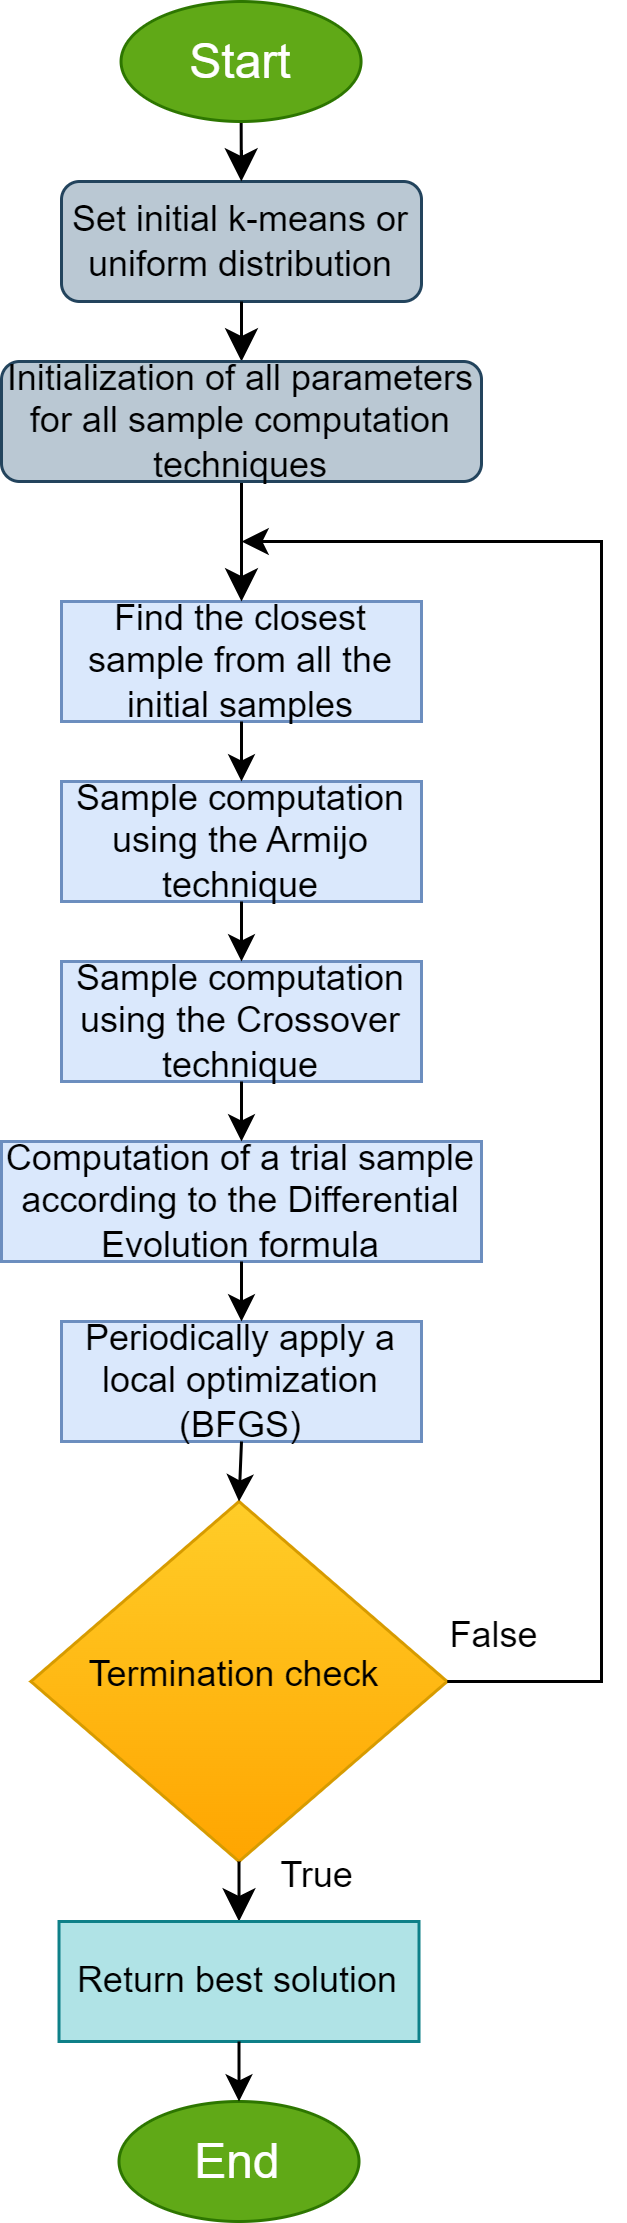
\includegraphics{hybridFlowChart}
\par\end{centering}
\caption{The flowchart of the proposed optimization process.\label{fig:flow}}

\end{figure}

The optimization method described in section \ref{sec:overallAlgorithm}
combines evolutionary techniques, such as differential evolution,
Armijo line search, and components of genetic algorithms, with the
aim of finding the optimal solution. Initially, the population size
and the dimensionality of the target function are defined, and the
population samples are generated randomly using a uniform or k-means
distribution. For each sample, the Euclidean distance (equation \ref{eq:nearestSamply})
to the other samples is calculated to identify the nearest one, followed
by an Armijo line search (equation \ref{eq:findSample}) to determine
the optimal movement direction for the initial sample. Subsequently,
a new offspring sample is created using a crossover process (equation
\ref{eq:makeChild}), combining the current sample with the best discovered
so far. A trial vector (equation \ref{eq:trialSample}) is then formed,
which accounts for the adjustment of the computed samples and the
differential coefficient parameter derived from the differential evolution
algorithm. Periodically, local search methods, such as BFGS\citep{bfgs},
are applied to improve the accuracy of the solution search. The method
terminates when the best solution found remains nearly unchanged for
a specified number of iterations. In summary, the basic steps for
calculating a new sample are:
\begin{itemize}
\item Identification of the nearest point \textbf{$c_{\iota}$ }for each
sample\textbf{ $x_{\iota}$}.
\item Calculation of a sample $\mbox{minLS}(x_{i},c_{i})$ through Armijo
line search, between the sample \textbf{$x_{i}$ }and the sample$c_{i}$.
\item Generation of the sample using the crossover process of the Genetic
Algorithm, between the sample \textbf{$x_{\iota}$ }and the best sample$x^{best}$
.
\item Computation of the trial point $y_{i}$ using a process derived from
Differential Evolution.
\end{itemize}

\section{Experiments\label{sec:Experiments}}

\subsection{Settings and benchmark functions}

The benchmark functions used in the experimental measurements are
presented in Table \ref{tab:benchmarkFunctions}. 
\begin{table}[H]
\caption{The benchmark functions used in the conducted experiments.\label{tab:benchmarkFunctions}}

\centering{}%
\begin{tabular}{|c|c|c|}
\hline 
{\footnotesize{}NAME} & {\scriptsize{}FORMULA} & {\scriptsize{}DIMENSION}\tabularnewline
\hline 
\hline 
{\footnotesize{}ACKLEY} & {\scriptsize{}$f(x)=-a\exp\left(-b\sqrt{\frac{1}{n}\sum_{i=1}^{n}x_{i}^{2}}\right)-\exp\left(\frac{1}{n}\sum_{i=1}^{n}\cos\left(cx_{i}\right)\right)+a+\exp(1)\quad a=20.0$} & {\scriptsize{}2}\tabularnewline
\hline 
{\footnotesize{}BF1} & {\scriptsize{}$f(x)=-20\exp\left(-b\sqrt{\frac{1}{n}\sum_{i=1}^{n}x_{i}^{2}}\right)-\exp\left(\frac{1}{n}\sum_{i=1}^{n}\cos\left(cx_{i}\right)\right)+20+\exp(1)$} & {\scriptsize{}2}\tabularnewline
\hline 
{\footnotesize{}BF1} & {\scriptsize{}$f(x)=x_{1}^{2}+2x_{2}^{2}-\frac{3}{10}\cos\left(3\pi x_{1}\right)-\frac{4}{10}\cos\left(4\pi x_{2}\right)+\frac{7}{10}$} & {\scriptsize{}2}\tabularnewline
\hline 
{\footnotesize{}BF2} & {\scriptsize{}$f(x)=x_{1}^{2}+2x_{2}^{2}-\frac{3}{10}\cos\left(3\pi x_{1}\right)\cos\left(4\pi x_{2}\right)+\frac{3}{10}$} & {\scriptsize{}2}\tabularnewline
\hline 
{\footnotesize{}BF3} & {\scriptsize{}$f(x)=x_{1}^{2}+2x_{2}^{2}-\frac{3}{10}\cos\left(3\pi x_{1}\right)\cos\left(4\pi x_{2}\right)+\frac{3}{10}$} & {\scriptsize{}2}\tabularnewline
\hline 
{\footnotesize{}DIFFPOWER} & {\scriptsize{}$f(x)=\sum_{i=1}^{n}|x_{i}-y_{i}|^{p}$} & {\scriptsize{}$n=2\ p=2,5,10$}\tabularnewline
\hline 
{\footnotesize{}CAMEL} & {\scriptsize{}$f(x)=4x_{1}^{2}-2.1x_{1}^{4}+\frac{1}{3}x_{1}^{6}+x_{1}x_{2}-4x_{2}^{2}+4x_{2}^{4},\quad x\in[-5,5]^{2}$} & {\scriptsize{}2}\tabularnewline
\hline 
{\footnotesize{}EASOM} & {\scriptsize{}$f(x)=-\cos\left(x_{1}\right)\cos\left(x_{2}\right)\exp\left(\left(x_{2}-\pi\right)^{2}-\left(x_{1}-\pi\right)^{2}\right)$} & {\scriptsize{}2}\tabularnewline
\hline 
{\footnotesize{}ELP} & {\scriptsize{}$f(x)=\sum_{i=1}^{n}\left(10^{6}\right)^{\frac{i-1}{n-1}}x_{i}^{2}$} & {\scriptsize{}$n=10,20,30$}\tabularnewline
\hline 
{\footnotesize{}EXP} & {\scriptsize{}$f(x)=-\exp\left(-0.5\sum_{i=1}^{n}x_{i}^{2}\right),\quad-1\le x_{i}\le1$} & {\scriptsize{}$n=4,8,16,32$}\tabularnewline
\hline 
{\footnotesize{}F3} & {\scriptsize{}$f(x)=\left(e^{-2.0\log(2.0)\left(\frac{(x_{1}-0.08)}{0.854}\right)^{2}}\right)\left(\sin\left(5.0\pi\left(x_{1}^{\frac{3.0}{4.0}}-0.05\right)\right)\right)^{6}\quad x\in[0,1]^{n}$} & {\scriptsize{}2}\tabularnewline
\hline 
{\footnotesize{}F5} & {\scriptsize{}$f(x)=\left(\left(4.0-2.1x_{1}^{2}+\frac{x_{1}^{4}}{3.0}\right)x_{1}^{2}\right)+\left(x_{1}x_{2}\right)+\left(\left(4.0x_{2}^{2}-4.0\right)x_{2}^{2}\right)\quad-5\le x_{i}\le5$} & {\scriptsize{}2}\tabularnewline
\hline 
{\footnotesize{}F9} & {\scriptsize{}$f(x)=-\exp\left(-0.5\sum_{i=1}^{n}x_{i}^{2}\right),\quad x\in[0,1]^{n}$} & {\scriptsize{}2}\tabularnewline
\hline 
{\footnotesize{}GKLS\citep{Gaviano}} & {\scriptsize{}$f(x)=\mbox{Gkls}(x,n,w)$} & {\scriptsize{}$n=2,3\ w=50,100$}\tabularnewline
\hline 
{\footnotesize{}GRIEWANK2} & {\scriptsize{}$f(x)=1+\frac{1}{200}\sum_{i=1}^{2}x_{i}^{2}-\prod_{i=1}^{2}\frac{\cos(x_{i})}{\sqrt{(i)}}$} & {\scriptsize{}2}\tabularnewline
\hline 
{\footnotesize{}GRIEWANK10} & {\scriptsize{}f$(x)=1+\frac{1}{200}\sum_{i=1}^{10}x_{i}^{2}-\prod_{i=1}^{10}\frac{\cos(x_{i})}{\sqrt{(i)}}$} & {\scriptsize{}10}\tabularnewline
\hline 
{\footnotesize{}HANSEN} & {\scriptsize{}$f(x)=\sum_{i=1}^{5}i\cos\left[(i-1)x_{1}+i\right]\sum_{j=1}^{5}j\cos\left[(j+1)x_{2}+j\right]$} & {\scriptsize{}2}\tabularnewline
\hline 
{\footnotesize{}HARTMAN3} & {\scriptsize{}$f(x)=-\sum_{i=1}^{4}c_{i}\exp\left(-\sum_{j=1}^{3}a_{ij}\left(x_{j}-p_{ij}\right)^{2}\right)$} & {\scriptsize{}3}\tabularnewline
\hline 
{\footnotesize{}HARTAMN6} & {\scriptsize{}$f(x)=-\sum_{i=1}^{4}c_{i}\exp\left(-\sum_{j=1}^{6}a_{ij}\left(x_{j}-p_{ij}\right)^{2}\right)$} & {\scriptsize{}6}\tabularnewline
\hline 
{\footnotesize{}POTENTIAL\citep{Lennard}} & {\scriptsize{}$V_{LJ}(r)=4\epsilon\left[\left(\frac{\sigma}{r}\right)^{12}-\left(\frac{\sigma}{r}\right)^{6}\right]$} & {\scriptsize{}$n=9,15,21,30$}\tabularnewline
\hline 
{\footnotesize{}RARSTIGIN} & {\scriptsize{}$f(x)=x_{1}^{2}+x_{2}^{2}-\cos(18x_{1})-\cos(18x_{2})$} & {\scriptsize{}2}\tabularnewline
\hline 
{\footnotesize{}ROSENBROCK} & {\tiny{}$f(x)=\sum_{i=1}^{n-1}\left(100\left(x_{i+1}-x_{i}^{2}\right)^{2}+\left(x_{i}-1\right)^{2}\right),\quad-30\le x_{i}\le30$} & {\scriptsize{}$n=4,8,16$}\tabularnewline
\hline 
{\footnotesize{}SCHWEFELH} & {\tiny{}$f(x)=\sum_{i=1}^{n}\left(\sum_{j=1}^{i}x_{j}\right)^{2}$} & {\scriptsize{}2}\tabularnewline
\hline 
{\footnotesize{}SCHWEFELH221} & {\tiny{}$f(x)=418.9829n+\sum_{i=1}^{n}-x_{i}\sin\left(\sqrt{\left|x_{i}\right|}\right)$} & {\scriptsize{}2}\tabularnewline
\hline 
{\footnotesize{}SCHWEFELH222} & {\tiny{}$f(x)=\sum_{i=1}^{n-1}\left(100\left(x_{i+1}-x_{i}^{2}\right)^{2}+\left(x_{i}-1\right)^{2}\right),\quad-30\le x_{i}\le30$} & {\scriptsize{}2}\tabularnewline
\hline 
{\footnotesize{}Shekel5} & {\scriptsize{}$f(x)=-\sum_{i=1}^{5}\frac{1}{(x-a_{i})(x-a_{i})^{T}+c_{i}}$} & {\scriptsize{}4}\tabularnewline
\hline 
{\footnotesize{}Shekel7} & {\scriptsize{}$f(x)=-\sum_{i=1}^{7}\frac{1}{(x-a_{i})(x-a_{i})^{T}+c_{i}}$} & {\scriptsize{}4}\tabularnewline
\hline 
{\footnotesize{}Shekel10} & {\scriptsize{}$f(x)=-\sum_{i=1}^{10}\frac{1}{(x-a_{i})(x-a_{i})^{T}+c_{i}}$} & {\scriptsize{}4}\tabularnewline
\hline 
{\footnotesize{}Sinusoidal\citep{Zabinsky}} & {\scriptsize{}$f(x)=-\left(2.5\prod_{i=1}^{n}\sin\left(x_{i}-z\right)+\prod_{i=1}^{n}\sin\left(5\left(x_{i}-z\right)\right)\right),\quad0\le x_{i}\le\pi$} & {\scriptsize{}$n=4,8$}\tabularnewline
\hline 
{\footnotesize{}Test2N} & {\scriptsize{}$f(x)=\frac{1}{2}\sum_{i=1}^{n}x_{i}^{4}-16x_{i}^{2}+5x_{i}$} & {\scriptsize{}$n=4,5,7$}\tabularnewline
\hline 
{\footnotesize{}Test30N} & {\scriptsize{}$\frac{1}{10}\sin^{2}\left(3\pi x_{1}\right)\sum_{i=2}^{n-1}\left(\left(x_{i}-1\right)^{2}\left(1+\sin^{2}\left(3\pi x_{i+1}\right)\right)\right)+\left(x_{n}-1\right)^{2}\left(1+\sin^{2}\left(2\pi x_{n}\right)\right)$} & {\scriptsize{}$n=3,4$}\tabularnewline
\hline 
\end{tabular}
\end{table}
 The functions used in the conducted experiments have been proposed
by various researchers \citep{Ali1,Floudas1} in the relevant literature.
For a more accurate comparison of the methods, efforts were made to
maintain certain parameter values at equal or similar levels. The
values for the parameters of the algorithm are presented in Table\ref{tab:settings},
along with some explanation of each parameter.
\begin{center}
\begin{table}[H]
\caption{Parameters of optimization methods settings\label{tab:settings}}

\centering{}%
\begin{tabular}{|c|c|c|}
\hline 
PARAMETER & VALUE & EXPLANATION\tabularnewline
\hline 
\hline 
$N$ & $200$ & Number of samples for all methods\tabularnewline
\hline 
$N_{k}$ & $200$ & Maximum number of iterations for all methods\tabularnewline
\hline 
$SR$ & $\left|f_{\mbox{min}}^{(k)}-f_{\mbox{min}}^{(k-1)}\right|$ & Best fitness: Stopping rule for all methods\tabularnewline
\hline 
$N_{t}$ & $12$ & Similarity max count for all methods\tabularnewline
\hline 
$LS$ & $0.05$\ $(5\%)$ & Local search rate for all methods\tabularnewline
\hline 
$F$ & $0.8$ & Differential weight for Differential Evolution\tabularnewline
\hline 
$CR$ & $0.9$ & Crossover Probability for Differential Evolution\tabularnewline
\hline 
$C_{1},C_{2}$ & $0.5$ & Parameters of PSO\tabularnewline
\hline 
$G_{c}$ & $0.1$\ $(10\%)$ & Crossover rate for Genetic Algorithm\tabularnewline
\hline 
$G_{m}$ & $0.05$\ $(5\%)$ & Mutation rate for Genetic Algorithm\tabularnewline
\hline 
\end{tabular}
\end{table}
\par\end{center}

\subsection{Experimental results}

In the random number generator, different seeds were used to ensure
the reliability of the experimental results, with the experiments
being repeated 30 times. This process of repetition aims to minimize
the likelihood of random errors and to enhance the validity of the
results. The experiments were conducted on a system with an AMD Ryzen
5950X processor and 128 GB of RAM, operating in a Linux-Debian environment.
Additionally, the open-source optimizer \textquotedbl GlobalOptimus\textquotedbl{}
was used, which is a fully developed optimizer and is available for
distribution via the link: \url{http://www.github.com/itsoulos/GlobalOptimus}
(accessed on 17 September 2024). In Table \ref{tab:mainTable}, the
average function calls for each method and every objective function
is presented. The following notation are used in the experimental
tables:
\begin{enumerate}
\item The column FUNCTION represents the name of the used objective problem.
\item \textbf{The column GENETIC represents the application of the Genetic
Algorithm to the objective problem\citep{genetic3}.}
\item \textbf{The PSO column represents the implementation of the classical
PSO algorithm as suggested by the literature\citep{pso_major}.}
\item \textbf{The column IPSO stands for the application of the Improved
PSO algorithm as suggested by Charilogis and Tsoulos \citep{charilogis}
to the objective problems.}
\item \textbf{The column DE represents the average function calls for the
Differential Evolution optimization technique\citep{key-6}.}
\item \textbf{The column GWO represents the average function calls for the
Gray Wolf optimization technique\citep{key-2}.}
\item \textbf{The column WOA represents the average function calls for the
Whale Optimization technique\citep{WOA}.}
\item \textbf{The column MEWOA stands for the application of the Improved
WOA algorithm as suggested by Shen Y. et al \citep{key-1}to the objective
problems.}
\item The total sum of calls for each method is listed at the end of the
table. 
\item The success rate is indicated by the number in parentheses, which
shows the executions in which the global optimum was successfully
found. The absence of this number implies that the global minimum
was computed with 100\% success in all independent runs.
\end{enumerate}
{\footnotesize{}}
\begin{table}[H]
\centering{}{\footnotesize{}\caption{Comparison of average function calls of proposed method against others\label{tab:mainTable}}
}%
\begin{tabular}{|>{\centering}V{\linewidth}|c|c|c|c|c|c|c|c|c|}
\hline 
{\tiny{}FUNCTION} & {\tiny{}GENETIC} & {\tiny{}PSO} & {\tiny{}IPSO} & {\tiny{}DE} & {\tiny{}GWO} & {\tiny{}WOA} & {\tiny{}MEWOA} & {\tiny{}PROPOSED} & {\tiny{}PROPOSED KMEANS}\tabularnewline
\hline 
\hline 
{\tiny{}ACKLEY} & {\tiny{}6749} & {\tiny{}6885} & {\tiny{}3418} & {\tiny{}16183} & {\tiny{}20182} & {\tiny{}24766} & {\tiny{}13879} & {\tiny{}5818} & {\tiny{}3490}\tabularnewline
\hline 
{\tiny{}BF1} & {\tiny{}4007} & {\tiny{}4113} & {\tiny{}1814} & {\tiny{}8268} & {\tiny{}9120} & {\tiny{}9924} & {\tiny{}7987} & {\tiny{}5585} & {\tiny{}3023}\tabularnewline
\hline 
{\tiny{}BF2} & {\tiny{}3793} & {\tiny{}3747} & {\tiny{}1759} & {\tiny{}7913} & {\tiny{}8731} & {\tiny{}9597} & {\tiny{}6262} & {\tiny{}5008} & {\tiny{}2693}\tabularnewline
\hline 
{\tiny{}BF3} & {\tiny{}3479} & {\tiny{}3305} & {\tiny{}1689} & {\tiny{}6327} & {\tiny{}7791} & {\tiny{}20117} & {\tiny{}5893} & {\tiny{}4282} & {\tiny{}2442}\tabularnewline
\hline 
{\tiny{}BRANIN} & {\tiny{}2376} & {\tiny{}2522} & {\tiny{}1730} & {\tiny{}4101} & {\tiny{}6055} & {\tiny{}5939} & {\tiny{}3367} & {\tiny{}3026} & {\tiny{}2087}\tabularnewline
\hline 
{\tiny{}CAMEL} & {\tiny{}2869} & {\tiny{}2908} & {\tiny{}1754} & {\tiny{}5609} & {\tiny{}6688} & {\tiny{}5917} & {\tiny{}4756} & {\tiny{}3327} & {\tiny{}2607}\tabularnewline
\hline 
{\tiny{}DIFFPOWER2} & {\tiny{}5443} & {\tiny{}8657} & {\tiny{}2462} & {\tiny{}14669} & {\tiny{}22059} & {\tiny{}11436} & {\tiny{}11536} & {\tiny{}8864} & {\tiny{}5617}\tabularnewline
\hline 
{\tiny{}DIFFPOWER5} & {\tiny{}18552} & {\tiny{}24894} & {\tiny{}4446} & {\tiny{}39018} & {\tiny{}49769} & {\tiny{}42095} & {\tiny{}31372} & {\tiny{}26065} & {\tiny{}17221}\tabularnewline
\hline 
{\tiny{}DIFFPOWER10} & {\tiny{}18801} & {\tiny{}32534} & {\tiny{}4690} & {\tiny{}46914} & {\tiny{}54442} & {\tiny{}56381} & {\tiny{}38559} & {\tiny{}29549} & {\tiny{}26615}\tabularnewline
\hline 
{\tiny{}EASOM} & {\tiny{}1958} & {\tiny{}1998} & {\tiny{}1753} & {\tiny{}2978} & {\tiny{}4615} & {\tiny{}3153} & {\tiny{}2455} & {\tiny{}2755} & {\tiny{}1402}\tabularnewline
\hline 
{\tiny{}ELP10} & {\tiny{}3131} & {\tiny{}4397} & {\tiny{}1720} & {\tiny{}6288} & {\tiny{}9415} & {\tiny{}10317} & {\tiny{}5255} & {\tiny{}4020} & {\tiny{}3593}\tabularnewline
\hline 
{\tiny{}ELP20} & {\tiny{}6160} & {\tiny{}6883} & {\tiny{}1988} & {\tiny{}10794} & {\tiny{}14173} & {\tiny{}17040} & {\tiny{}7722} & {\tiny{}6537} & {\tiny{}6194}\tabularnewline
\hline 
{\tiny{}ELP30} & {\tiny{}9576} & {\tiny{}9438} & {\tiny{}2100} & {\tiny{}14172} & {\tiny{}18245} & {\tiny{}23532} & {\tiny{}9776} & {\tiny{}8270} & {\tiny{}3593}\tabularnewline
\hline 
{\tiny{}EXP4} & {\tiny{}2946} & {\tiny{}3177} & {\tiny{}1677} & {\tiny{}5166} & {\tiny{}6648} & {\tiny{}5567} & {\tiny{}4392} & {\tiny{}3570} & {\tiny{}2238}\tabularnewline
\hline 
{\tiny{}EXP16} & {\tiny{}3250} & {\tiny{}3477} & {\tiny{}1660} & {\tiny{}6498} & {\tiny{}6978} & {\tiny{}9968} & {\tiny{}4624} & {\tiny{}3854} & {\tiny{}3588}\tabularnewline
\hline 
{\tiny{}EXP32} & {\tiny{}3561} & {\tiny{}3728} & {\tiny{}1647} & {\tiny{}7606} & {\tiny{}7419} & {\tiny{}11925} & {\tiny{}4508} & {\tiny{}3852} & {\tiny{}3691}\tabularnewline
\hline 
{\tiny{}F3} & {\tiny{}4074} & {\tiny{}3420} & {\tiny{}1979(50)} & {\tiny{}7323} & {\tiny{}10816} & {\tiny{}11717} & {\tiny{}5821} & {\tiny{}6444} & {\tiny{}5434}\tabularnewline
\hline 
{\tiny{}F5} & {\tiny{}1630} & {\tiny{}2055} & {\tiny{}1376} & {\tiny{}2814} & {\tiny{}48377} & {\tiny{}7393} & {\tiny{}2117} & {\tiny{}2697} & {\tiny{}2199}\tabularnewline
\hline 
{\tiny{}F9} & {\tiny{}2494} & {\tiny{}2707} & {\tiny{}1879} & {\tiny{}4535} & {\tiny{}5502} & {\tiny{}4479} & {\tiny{}3534} & {\tiny{}4406} & {\tiny{}1968}\tabularnewline
\hline 
{\tiny{}GKLS250} & {\tiny{}2280} & {\tiny{}2495} & {\tiny{}1623} & {\tiny{}3834} & {\tiny{}6127} & {\tiny{}4978} & {\tiny{}3665} & {\tiny{}2315} & {\tiny{}1657}\tabularnewline
\hline 
{\tiny{}GKLS350} & {\tiny{}2612} & {\tiny{}2658} & {\tiny{}1570} & {\tiny{}3919} & {\tiny{}6919} & {\tiny{}7226(96)} & {\tiny{}3692} & {\tiny{}2265(96)} & {\tiny{}1335}\tabularnewline
\hline 
{\tiny{}GOLDSTEIN} & {\tiny{}3687} & {\tiny{}3856} & {\tiny{}1886} & {\tiny{}6781} & {\tiny{}9312} & {\tiny{}9016} & {\tiny{}5287} & {\tiny{}3930} & {\tiny{}2727}\tabularnewline
\hline 
{\tiny{}GRIEWANK2} & {\tiny{}4500} & {\tiny{}3168} & {\tiny{}2299(96)} & {\tiny{}7429(96)} & {\tiny{}9253} & {\tiny{}7948(86)} & {\tiny{}7285} & {\tiny{}3850(50)} & {\tiny{}2223}\tabularnewline
\hline 
{\tiny{}GRIEWANK10} & {\tiny{}6409(96)} & {\tiny{}7942} & {\tiny{}2142(80)} & {\tiny{}18490} & {\tiny{}14708} & {\tiny{}51143} & {\tiny{}12341} & {\tiny{}7551} & {\tiny{}6593}\tabularnewline
\hline 
{\tiny{}HANSEN} & {\tiny{}3209} & {\tiny{}2892} & {\tiny{}2204} & {\tiny{}4185} & {\tiny{}7253} & {\tiny{}10498} & {\tiny{}4116} & {\tiny{}4565} & {\tiny{}3092}\tabularnewline
\hline 
{\tiny{}HARTMAN3} & {\tiny{}2751} & {\tiny{}3103} & {\tiny{}1801} & {\tiny{}5190} & {\tiny{}7293} & {\tiny{}8440} & {\tiny{}3982} & {\tiny{}3145} & {\tiny{}2100}\tabularnewline
\hline 
{\tiny{}HARTMAN6} & {\tiny{}3219} & {\tiny{}3688} & {\tiny{}1862} & {\tiny{}5968} & {\tiny{}8814} & {\tiny{}22615} & {\tiny{}4416} & {\tiny{}4105} & {\tiny{}2921}\tabularnewline
\hline 
{\tiny{}POTENTIAL3} & {\tiny{}4351} & {\tiny{}5154} & {\tiny{}3096} & {\tiny{}6218} & {\tiny{}11256} & {\tiny{}9232} & {\tiny{}5071} & {\tiny{}4790} & {\tiny{}4034}\tabularnewline
\hline 
{\tiny{}POTENTIAL5} & {\tiny{}7704} & {\tiny{}10128} & {\tiny{}6353} & {\tiny{}9119} & {\tiny{}22136} & {\tiny{}39455} & {\tiny{}8807} & {\tiny{}7995} & {\tiny{}7991}\tabularnewline
\hline 
{\tiny{}POTENTIAL6} & {\tiny{}10177(70)} & {\tiny{}11780(46)} & {\tiny{}7593} & {\tiny{}10509} & {\tiny{}32630(90)} & {\tiny{}46466(46)} & {\tiny{}11341(76)} & {\tiny{}8906(76)} & {\tiny{}9333(76)}\tabularnewline
\hline 
{\tiny{}POTENTIAL10} & {\tiny{}13357} & {\tiny{}16550(86)} & {\tiny{}10413} & {\tiny{}12721} & {\tiny{}38337} & {\tiny{}59487} & {\tiny{}18573} & {\tiny{}12757} & {\tiny{}13611}\tabularnewline
\hline 
{\tiny{}RASTRIGIN} & {\tiny{}4106} & {\tiny{}3539} & {\tiny{}2211} & {\tiny{}6216} & {\tiny{}9043} & {\tiny{}8116} & {\tiny{}5523} & {\tiny{}3672(86)} & {\tiny{}2364}\tabularnewline
\hline 
{\tiny{}ROSENBROCK4} & {\tiny{}3679} & {\tiny{}5858} & {\tiny{}2025} & {\tiny{}8452} & {\tiny{}8078} & {\tiny{}10759} & {\tiny{}7750} & {\tiny{}5642} & {\tiny{}3641}\tabularnewline
\hline 
{\tiny{}ROSENBROCK8} & {\tiny{}5269} & {\tiny{}7843} & {\tiny{}2085} & {\tiny{}11530} & {\tiny{}11167} & {\tiny{}14094} & {\tiny{}9469} & {\tiny{}7926} & {\tiny{}6119}\tabularnewline
\hline 
{\tiny{}ROSENBROCK16} & {\tiny{}8509} & {\tiny{}11450} & {\tiny{}2432} & {\tiny{}17432} & {\tiny{}15590} & {\tiny{}23544} & {\tiny{}13554} & {\tiny{}11285} & {\tiny{}7490}\tabularnewline
\hline 
{\tiny{}SCHWEFEL} & {\tiny{}1880} & {\tiny{}2178} & {\tiny{}1504} & {\tiny{}3437} & {\tiny{}4564} & {\tiny{}4158} & {\tiny{}3005} & {\tiny{}2208} & {\tiny{}1572}\tabularnewline
\hline 
{\tiny{}SCHWEFEL221} & {\tiny{}2666} & {\tiny{}2529(70)} & {\tiny{}1875(70)} & {\tiny{}3909} & {\tiny{}71847} & {\tiny{}8519(96)} & {\tiny{}3815} & {\tiny{}2867} & {\tiny{}2256}\tabularnewline
\hline 
{\tiny{}SCHWEFEL222} & {\tiny{}33724} & {\tiny{}42897} & {\tiny{}28965} & {\tiny{}86861} & {\tiny{}101960} & {\tiny{}114161} & {\tiny{}65835} & {\tiny{}78734} & {\tiny{}18058}\tabularnewline
\hline 
{\tiny{}SHEKEL5} & {\tiny{}3325} & {\tiny{}3886} & {\tiny{}2018} & {\tiny{}6662} & {\tiny{}10043} & {\tiny{}17010} & {\tiny{}5359} & {\tiny{}5322} & {\tiny{}2657}\tabularnewline
\hline 
{\tiny{}SHEKEL7} & {\tiny{}3360} & {\tiny{}4009} & {\tiny{}1994} & {\tiny{}6967(76)} & {\tiny{}10079} & {\tiny{}17873} & {\tiny{}5344} & {\tiny{}5503} & {\tiny{}2648}\tabularnewline
\hline 
{\tiny{}SHEKEL10} & {\tiny{}2488} & {\tiny{}3985} & {\tiny{}1914(96)} & {\tiny{}6757(96)} & {\tiny{}10055} & {\tiny{}15524} & {\tiny{}5321} & {\tiny{}4784} & {\tiny{}2901}\tabularnewline
\hline 
{\tiny{}SINU4} & {\tiny{}2990} & {\tiny{}3409} & {\tiny{}1961} & {\tiny{}5953} & {\tiny{}8132} & {\tiny{}10150} & {\tiny{}4874} & {\tiny{}3446} & {\tiny{}2254}\tabularnewline
\hline 
{\tiny{}SINU8} & {\tiny{}3441} & {\tiny{}3995} & {\tiny{}1853} & {\tiny{}6973} & {\tiny{}10481} & {\tiny{}20782} & {\tiny{}5586} & {\tiny{}4371} & {\tiny{}3359}\tabularnewline
\hline 
{\tiny{}SINU16} & {\tiny{}4320} & {\tiny{}4680} & {\tiny{}2251} & {\tiny{}6979} & {\tiny{}15356} & {\tiny{}34409} & {\tiny{}7274} & {\tiny{}6450} & {\tiny{}5992}\tabularnewline
\hline 
{\tiny{}TEST2N4} & {\tiny{}3330} & {\tiny{}3390} & {\tiny{}1930} & {\tiny{}6396} & {\tiny{}8093} & {\tiny{}11876(96)} & {\tiny{}4930} & {\tiny{}3569} & {\tiny{}2204}\tabularnewline
\hline 
{\tiny{}TEST2N5} & {\tiny{}4000} & {\tiny{}3604} & {\tiny{}1982(93)} & {\tiny{}6271(96)} & {\tiny{}8812} & {\tiny{}16256(86)} & {\tiny{}5045} & {\tiny{}3877(93)} & {\tiny{}2575(93)}\tabularnewline
\hline 
{\tiny{}TEST2N7} & {\tiny{}4775} & {\tiny{}4020(96)} & {\tiny{}2157(73)} & {\tiny{}7074(73)} & {\tiny{}10124} & {\tiny{}25005(63)} & {\tiny{}6363(93)} & {\tiny{}4285(50)} & {\tiny{}2831(36)}\tabularnewline
\hline 
{\tiny{}TEST30N3} & {\tiny{}3210} & {\tiny{}4018} & {\tiny{}2432} & {\tiny{}6178} & {\tiny{}7647} & {\tiny{}8163} & {\tiny{}5311} & {\tiny{}4215} & {\tiny{}4389}\tabularnewline
\hline 
{\tiny{}TEST30N4} & {\tiny{}3678} & {\tiny{}4504} & {\tiny{}3354} & {\tiny{}7006} & {\tiny{}10656} & {\tiny{}13596} & {\tiny{}7069} & {\tiny{}5013} & {\tiny{}2901}\tabularnewline
\hline 
{\tiny{}TOTAL} & {\tiny{}261106} & {\tiny{}317168} & {\tiny{}145908} & {\tiny{}506409} & {\tiny{}802608} & {\tiny{}916996} & {\tiny{}419939} & {\tiny{}361454} & {\tiny{}230033}\tabularnewline
\hline 
\end{tabular}
\end{table}
 At the end of every global optimization procedure, a BFGS variant
of Powell \citep{powell} is utilized to improve the discovered solution
and identify with certainty a local minimum.  Additionally, Figure
\ref{fig:proposedVSOthers} presents a statistical comparison between
the used optimization methods and the data provided from Table \ref{tab:mainTable}.

\begin{figure}[H]
\centering{}\subfloat[With outliers appearing\label{fig:CompWith}]{
\begin{centering}
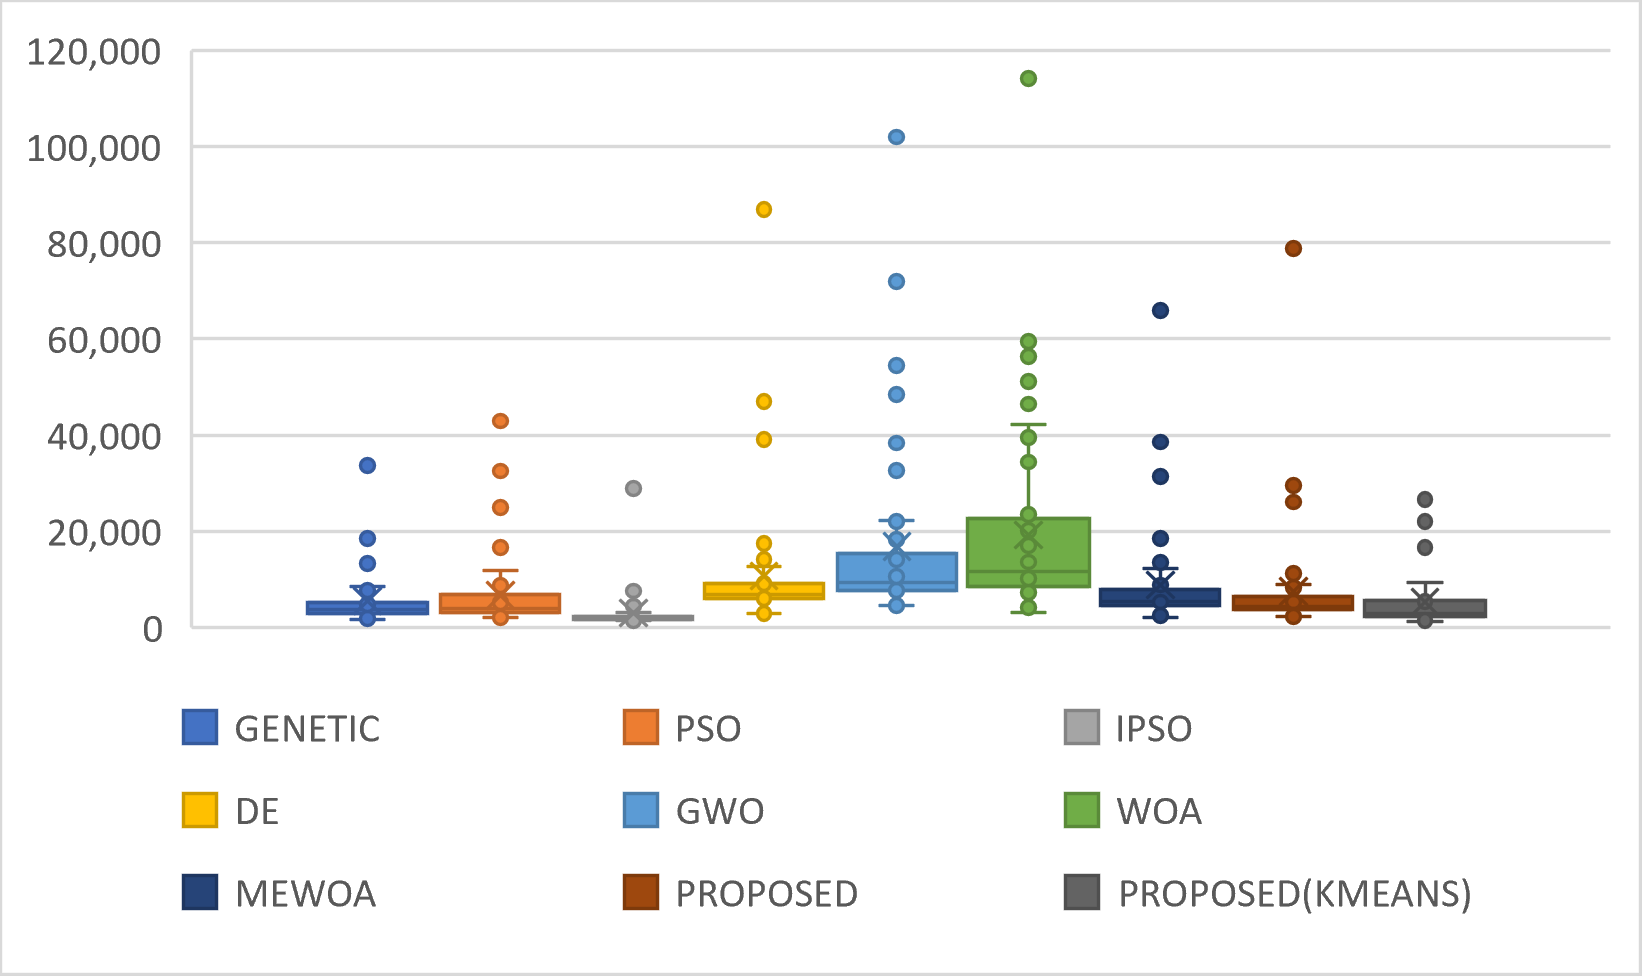
\includegraphics[scale=0.4]{new10}
\par\end{centering}
}\subfloat[Without outliers appearing\label{fig:CompWithout}]{\begin{centering}
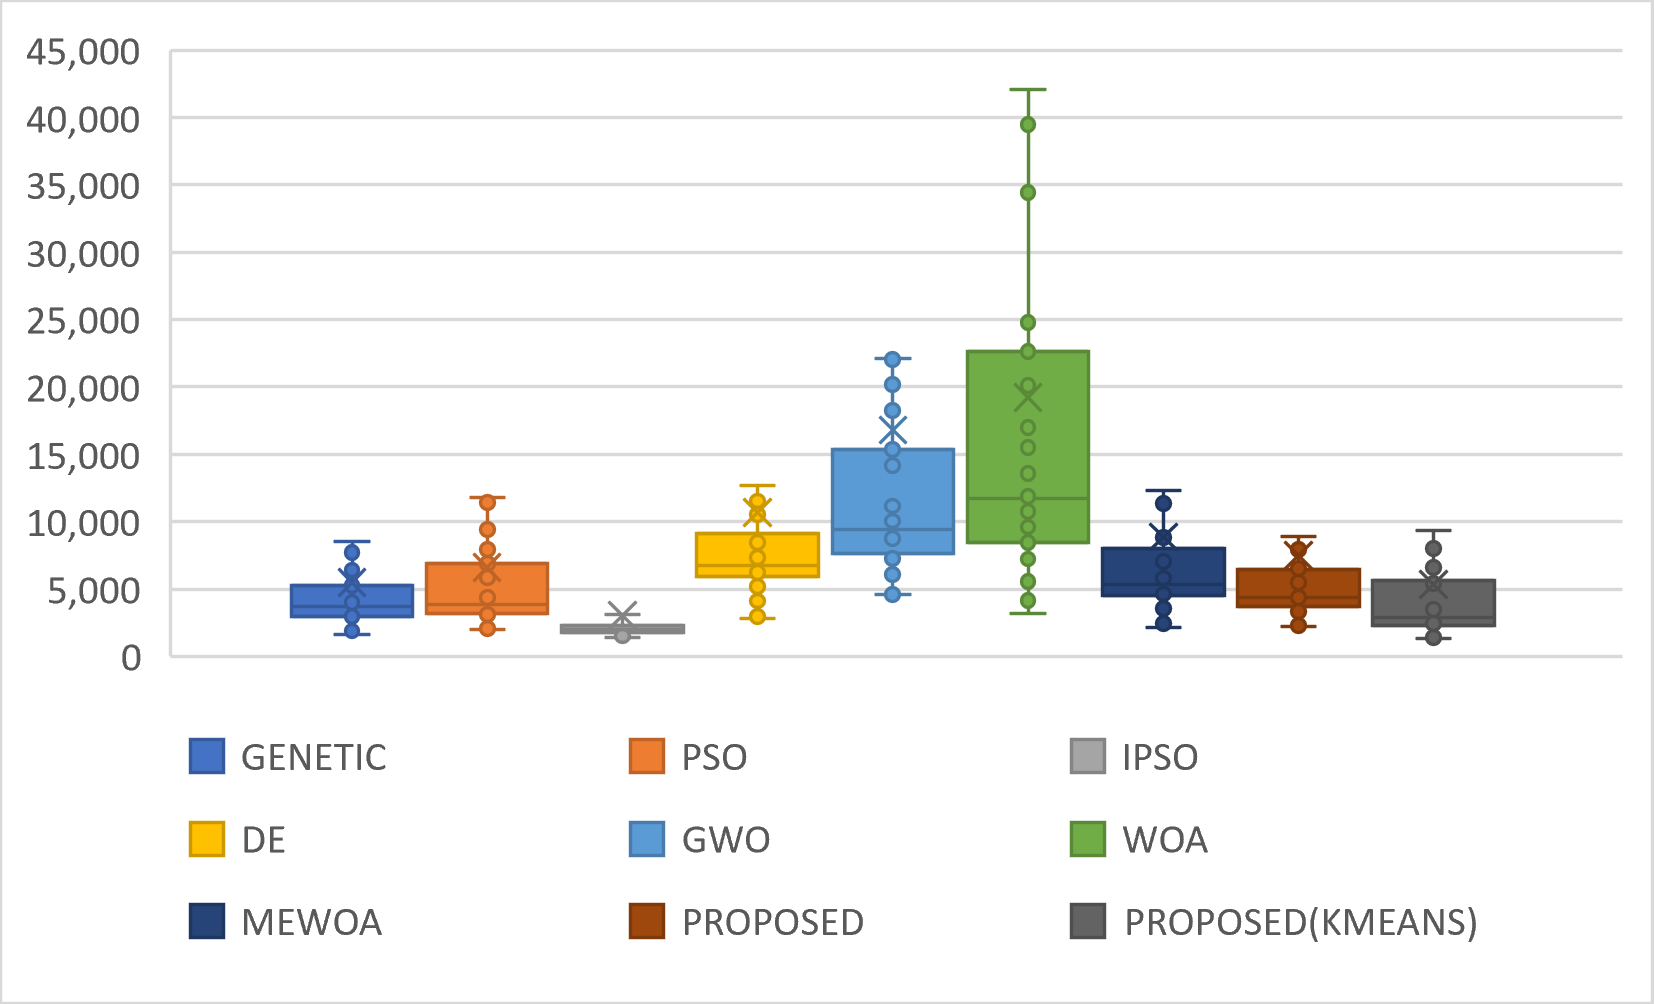
\includegraphics[scale=0.4]{new11}
\par\end{centering}
}\caption{Comparison of function calls of proposed method against others\label{fig:proposedVSOthers}}
\end{figure}
 

\begin{figure}[H]
\centering{}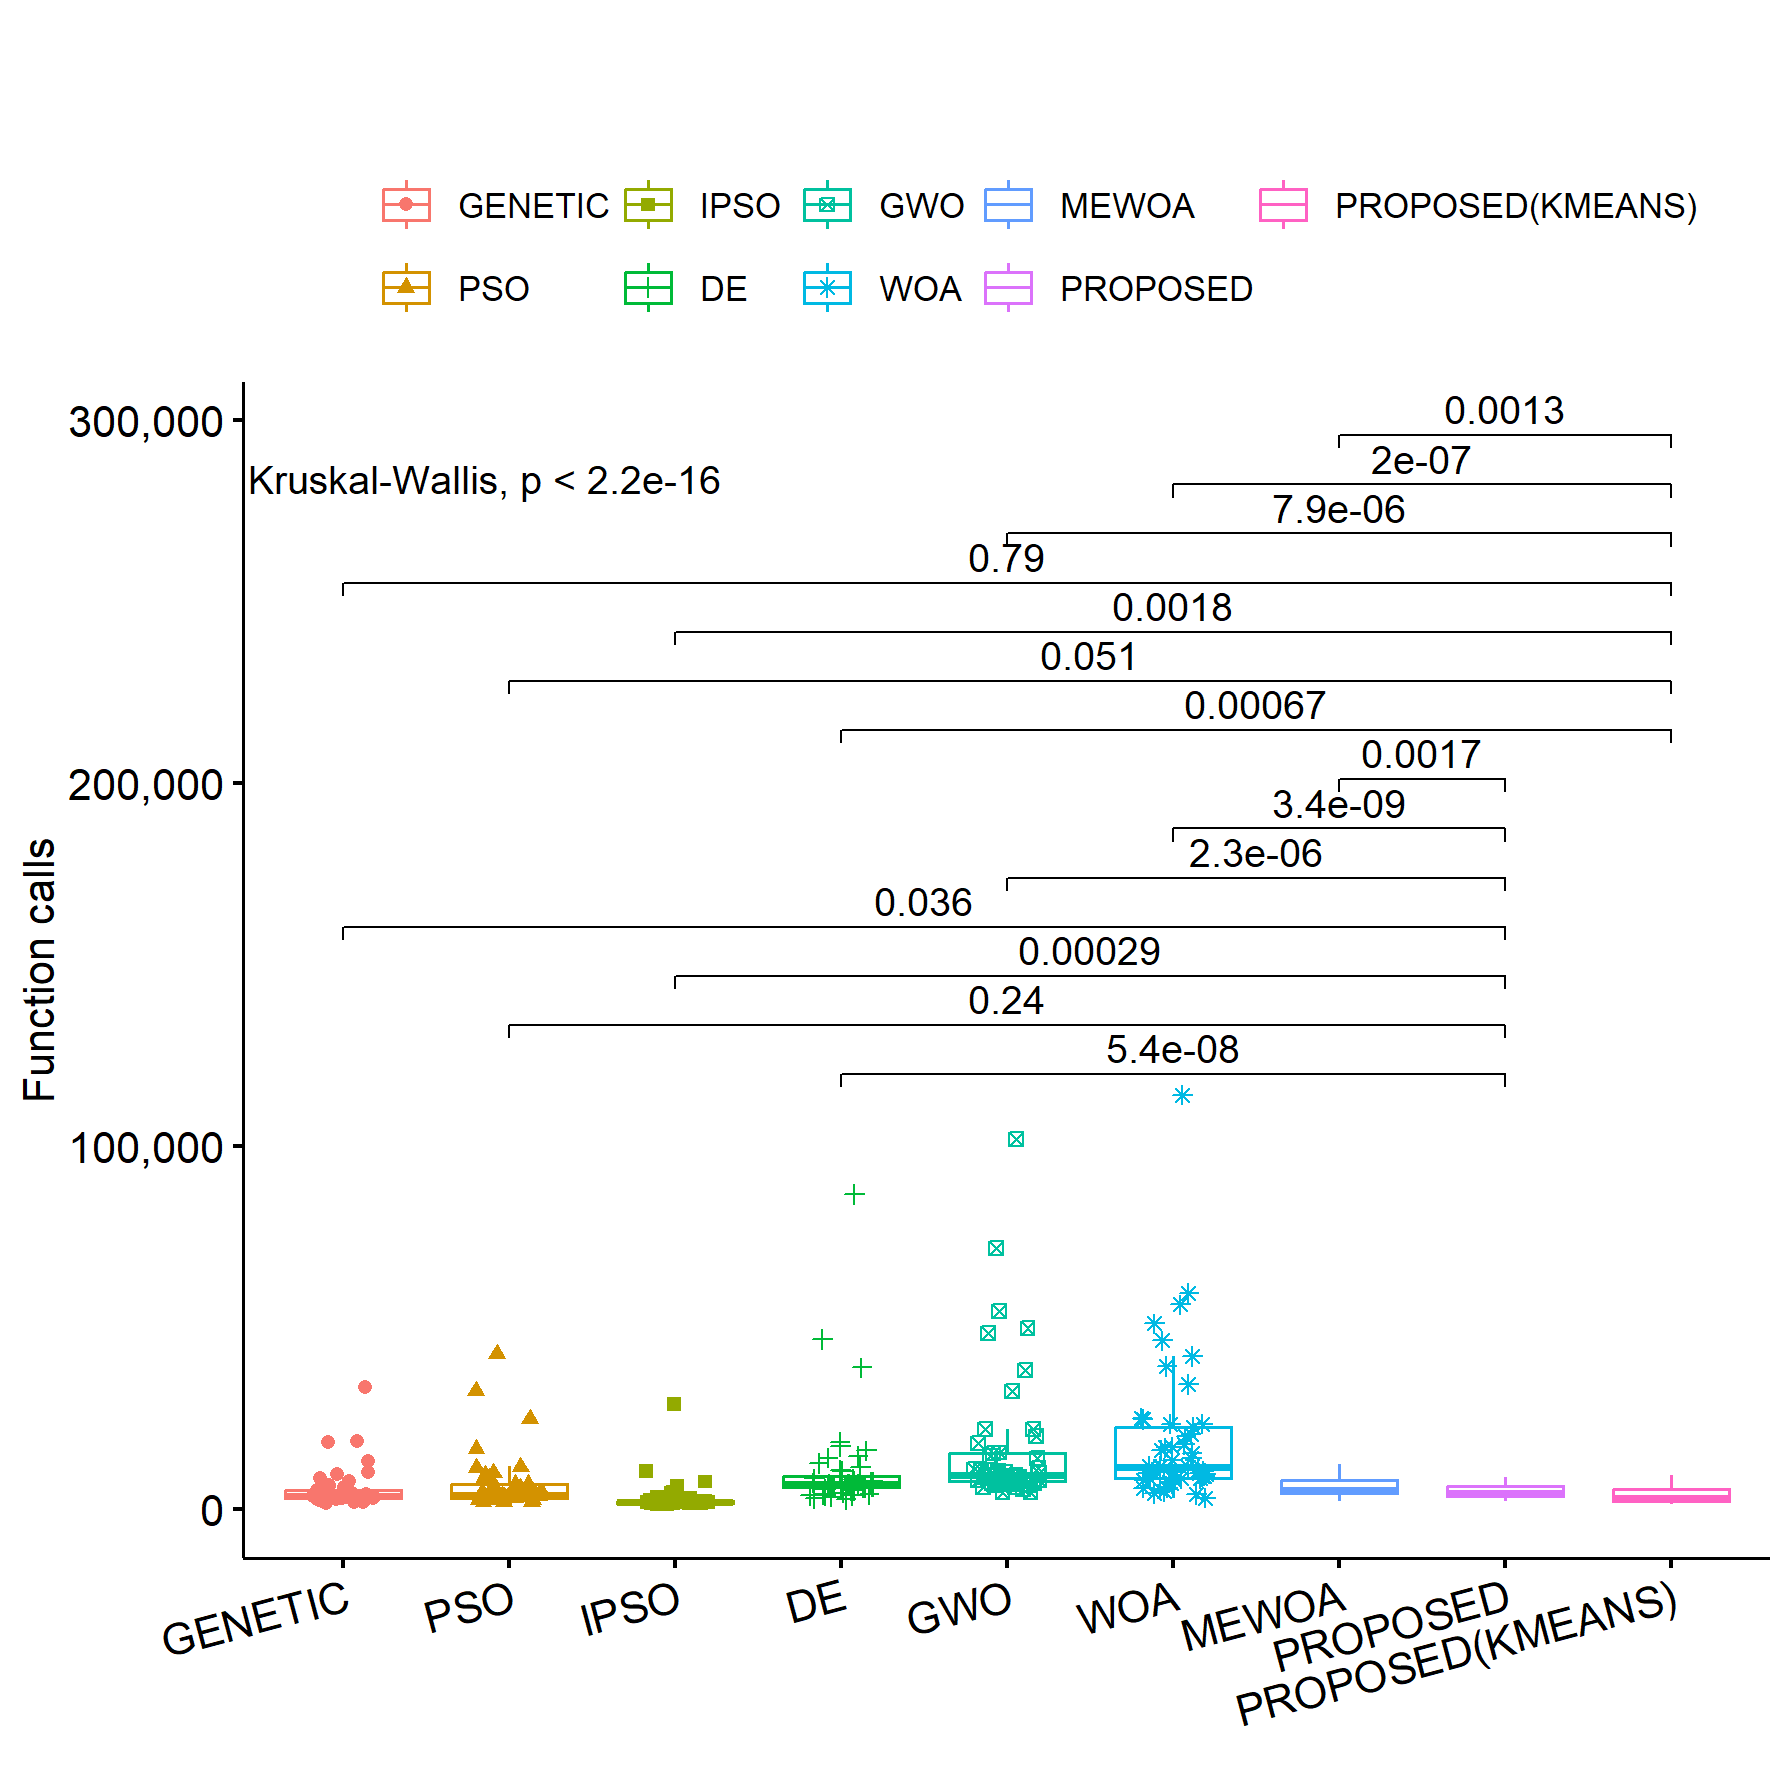
\includegraphics[scale=0.5]{new12}\caption{Statistical comparison of proposed method against others\label{fig:StatProposedVSOthers}}
\end{figure}

The table \ref{tab:mainTable} contains values representing objective
function evaluations, with lower values indicating better performance.
The goal is to minimize the number of function calls required to achieve
a result. The algorithms analyzed are GENETIC, PSO, IPSO, DE, GWO,
WOA, MEWOA, PROPOSED, and PROPOSED(KMEANS). The GENETIC algorithm,
with a total of 261,106 evaluations, shows mixed results. In some
functions, such as SHEKEL10 with 2488 evaluations, it performs well.
However, in more demanding functions, like DIFFPOWER5 and DIFFPOWER10
with 18,552 and 18,801 evaluations respectively, it requires many
calls, indicating reduced efficiency. The PSO algorithm, with 317,168
total evaluations, needs more calls than GENETIC and is generally
considered less efficient. In difficult functions, such as DIFFPOWER10,
it requires many evaluations, indicating reduced effectiveness. The
IPSO algorithm is the most efficient, with only 145,908 evaluations.
Its low values in several functions, such as ROSENBROCK16 with 2432
calls and TEST2N5 with 1982 calls, indicate that it requires fewer
evaluations to achieve a result, making it the most efficient algorithm.
The DE algorithm, with 506,409 evaluations, performs worse compared
to IPSO and other algorithms. In difficult functions, such as DIFFPOWER10
with 46,914 calls and SCHWEFEL222 with 86,861 calls, it requires significantly
more evaluations, indicating difficulties in optimizing efficiently.
GWO has the most total evaluations (802,608), showing reduced efficiency.
It encounters particular difficulties in hard problems, such as DIFFPOWER10
with 54,442 calls and SCHWEFEL222 with 101,960 calls. WOA, with 916,996
evaluations, is even less efficient than GWO. It faces serious issues
in demanding functions such as DIFFPOWER10 (56,381 calls) and SCHWEFEL222
(114,161 calls), indicating poor performance. MEWOA (Modified WOA)
has 419,939 total evaluations, showing some improvement over WOA but
still less efficient than IPSO and PROPOSED+KMEANS. Despite the improvement,
it continues to require many calls in difficult problems, such as
DIFFPOWER10 (38,559 calls) and SCHWEFEL222 (65,835 calls). The PROPOSED
algorithm, with 361,454 evaluations, performs better than DE but does
not reach the efficiency of IPSO. It shows moderate results in some
problems, such as DIFFPOWER10 with 29,549 calls, limiting its overall
performance. The improved PROPOSED(KMEANS) algorithm achieves better
results, with 257,033 total evaluations. In many functions, such as
SCHWEFEL222 with 22,058 evaluations and DIFFPOWER10 with 26,615 evaluations,
the addition of KMEANS significantly improves performance, making
it competitive with IPSO. In conclusion, IPSO is the most efficient
algorithm, with the lowest total number of evaluations, achieving
better results with fewer calls. PROPOSED(KMEANS) also performs well,
approaching the performance of IPSO. On the other hand, GWO and WOA
have the worst performance, requiring the highest number of evaluations.
MEWOA shows some improvements over WOA but remains less efficient
than the top-performing algorithms.

In Figure {[}fig:StatProposedVSOthers{]}, pairwise comparisons between
the proposed methods and the other methods are presented. In all these
comparisons, the critical parameter p<0.05 confirms the statistical
significance of the results.

Overall, the proposed methods achieve a significant reduction in the
required number of objective function calls and, in many cases, outperform
other optimization techniques. Compared to the Differential Evolution
(DE) algorithm, the proposed approaches perform better across all
mathematical models, with the reduction in the number of calls exceeding
50\%. This trend is confirmed by Table \ref{tab:mainTable}. Additionally,
Figures \ref{fig:CompWith}, \ref{fig:CompWithout}, and \ref{fig:StatProposedVSOthers}
present statistical comparisons between the global optimization methods
used in the experiments, highlighting the superiority of the proposed
approaches.

An additional experiment was executed for the High Elliptic function,
which is defined as:
\[
f(x)=\sum_{i=1}^{n}\left(10^{6}\right)^{\frac{i-1}{n-1}}x_{i}^{2}
\]
where the parameter $n$ defines the dimension of the function. In
this particular experiment, the proposed optimization method was systematically
applied to a specific mathematical function as the dimension $n$
underwent a transition from 10 to 100. Figure \ref{fig:ELPcalls}
presents the number of objective function calls required for each
algorithm across different dimensions. As the problem dimension increases,
the number of function calls needed to find a solution grows significantly
for all algorithms, indicating the increasing complexity of the ELP
function. For example, the PROPOSED(KMEANS) algorithm requires 3593
calls for 10 dimensions and 20,900 calls for 100 dimensions, showing
a gradual increase. Similarly, the PROPOSED algorithm starts with
4020 calls for 10 dimensions and reaches 24,322 calls for 100 dimensions.
IPSO stands out as the most efficient algorithm, with only 1720 calls
at 10 dimensions and 3165 at 100, consistently maintaining low evaluations.
In contrast, WOA exhibits the worst performance, with 10,317 calls
at 10 dimensions and 62,878 at 100 dimensions. The rate of increase
in calls varies among algorithms. For example, the PROPOSED algorithm
increases from 4020 to 6537 calls between 10 and 20 dimensions (a
1.6 times increase), while the rise from 90 to 100 dimensions is more
moderate, from 20,798 to 24,322 calls. MEWOA, although improved compared
to WOA, requires more calls than the proposed methods, with 5255 calls
at 10 dimensions and 26,684 at 100. GENETIC displays a variable pattern,
with 3131 calls at 10 dimensions and 29,004 at 100. GWO and PSO follow
a similar trend, with a gradual increase in calls as the dimension
increases. Additionally, Figure \ref{fig:ELPTimes} illustrates the
execution time for each algorithm across different dimensions, measured
in seconds. As expected, increasing the dimension leads to a significant
rise in execution time for all algorithms, highlighting the increased
computational load. For example, PROPOSED(KMEANS) starts with 0.652
seconds at 10 dimensions and reaches 23.54 seconds at 100. PROPOSED
begins with 0.236 seconds at 10 dimensions and climbs to 32.784 seconds
at 100, marking an impressive 139-fold increase. The fastest algorithm,
IPSO, takes only 0.034 seconds at 10 dimensions and 2.106 seconds
at 100, demonstrating excellent performance and scalability. On the
other hand, WOA records the worst performance, with 75.319 seconds
at 100 dimensions compared to 0.257 seconds at 10 dimensions. DE also
struggles in execution time, increasing from 0.16 seconds at 10 dimensions
to 47.68 seconds at 100. The increase in execution time across dimensions
follows a nonlinear trend for most algorithms. For example, PROPOSED
takes 0.587 seconds at 20 dimensions (more than double the 0.236 seconds
at 10 dimensions) but reaches 14.847 seconds at 80 dimensions. Similarly,
PSO starts at 0.128 seconds at 10 dimensions and reaches 20.361 seconds
at 100 dimensions. 

The data reveals significant differences in the scalability and efficiency
of the algorithms. IPSO stands out as the most efficient algorithm,
with the lowest number of calls and the shortest execution time. PROPOSED(KMEANS)
also achieves satisfactory results, maintaining a balance between
calls and execution time. On the other hand, WOA and GWO exhibit the
worst performance, with significantly more calls and substantial increases
in execution time as the dimension grows.

The results confirm that the complexity of optimization problems increases
sharply with the dimension. Most algorithms struggle to maintain their
efficiency in higher dimensions, highlighting the importance of selecting
the appropriate algorithm according to the problem's requirements
and the available computational resources.
\begin{center}
\begin{figure}[H]
\begin{centering}
\subfloat[Function calls\label{fig:ELPcalls}]{\centering{}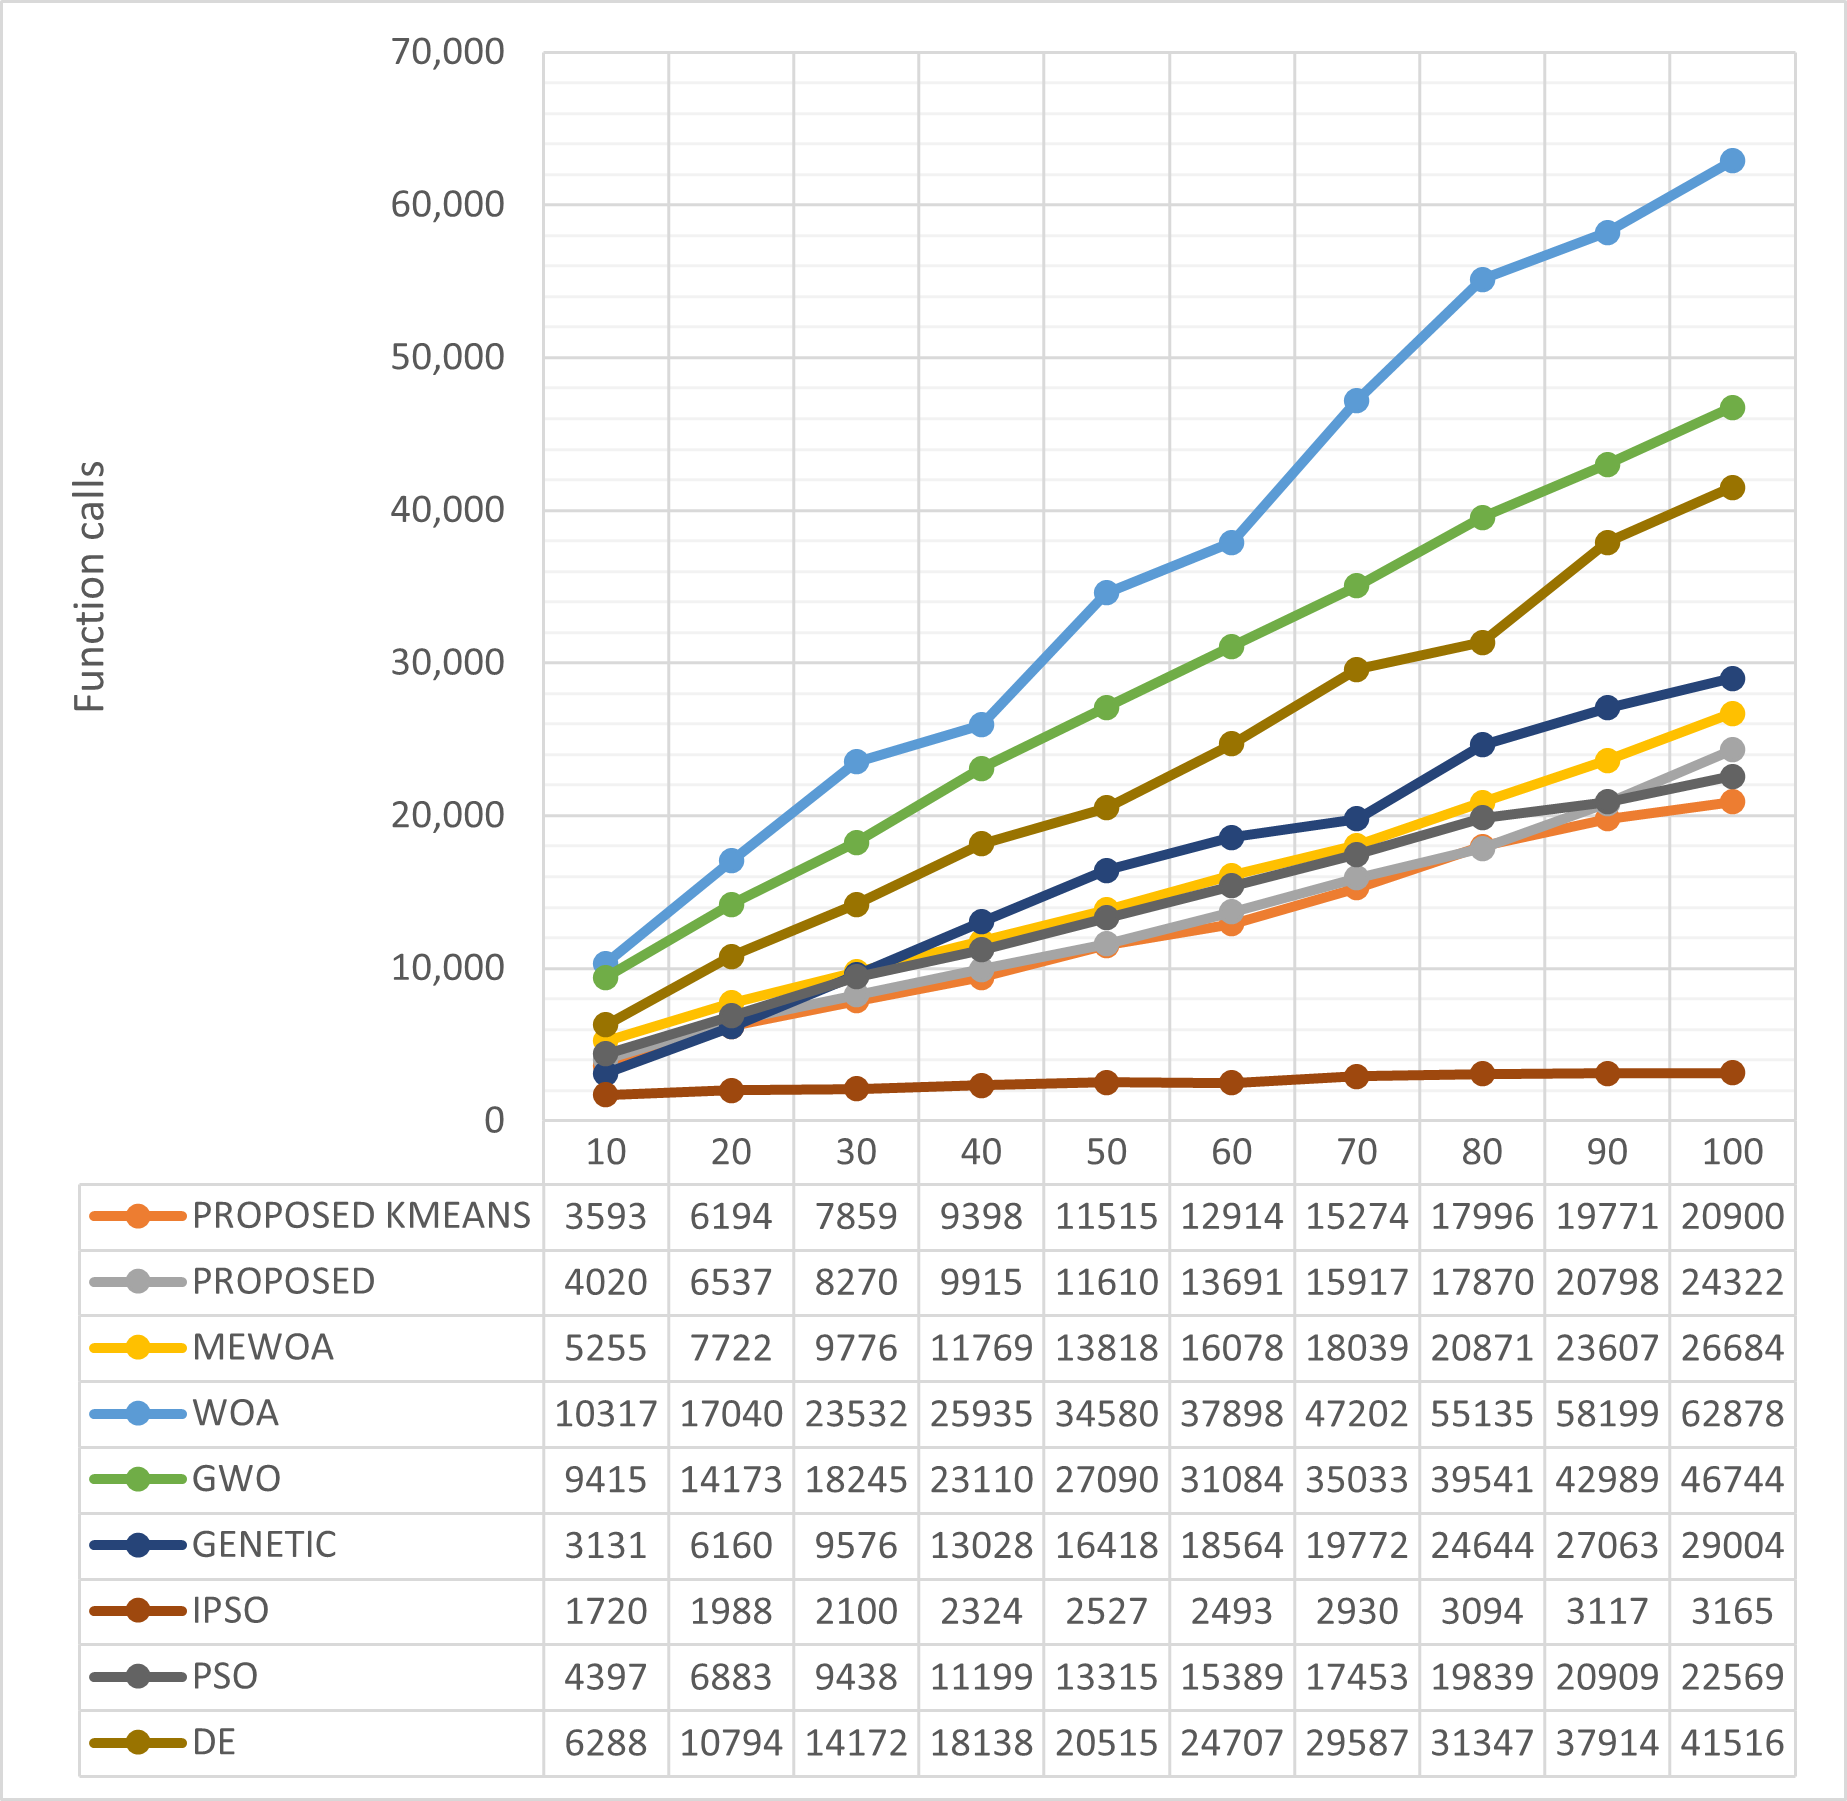
\includegraphics[scale=0.4]{new13}}\subfloat[Times\label{fig:ELPTimes}]{\begin{centering}
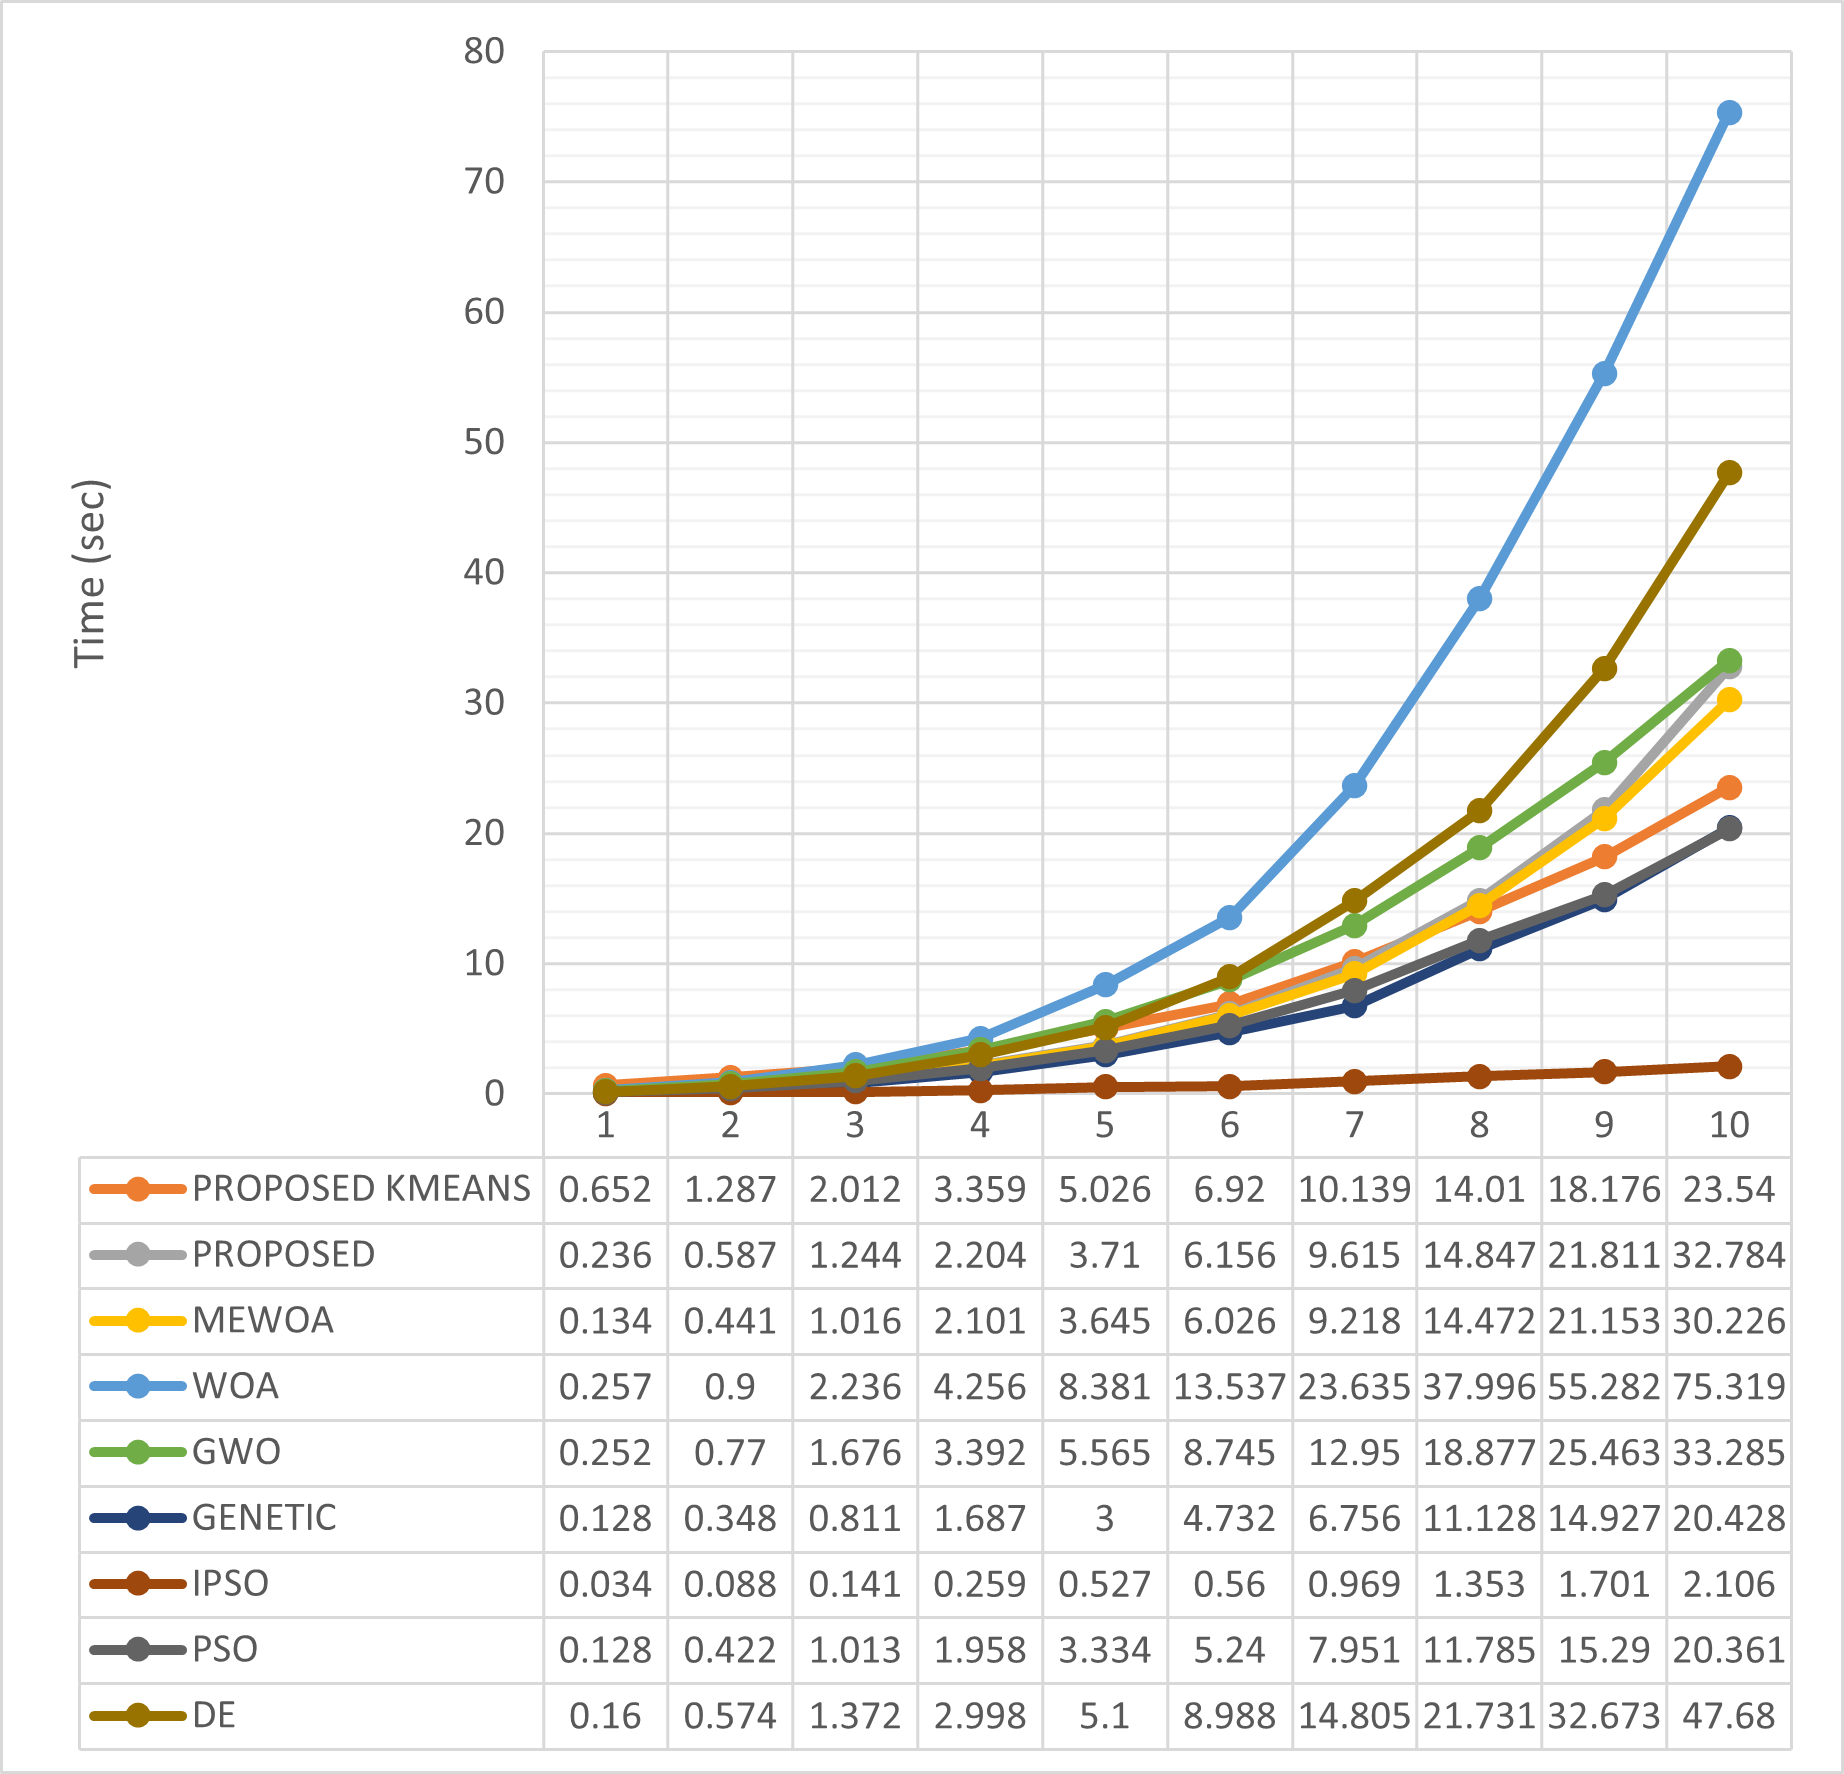
\includegraphics[scale=0.4]{new14}
\par\end{centering}
}\caption{Different variations of the ELP problem\label{fig:ELP}}
\par\end{centering}
\end{figure}
\par\end{center}

In each iteration of the algorithm, a trial point is calculated through
vector operations, similar to the process of optimization using differential
evolution. The main difference between the proposed method compared
to differential evolution lies in the fact that the samples for calculating
the trial point are selected from nearby regions of the initial distribution,
rather than being chosen randomly. However, the performance of the
two methods differs in their ability to find optimal solutions, as
shown in Figure\ref{fig:proposedsVSDE}. In the case where the initial
distribution is created by the k-means algorithm, the performance
increases by 36.3\%. The statistical analysis of the results in Figure
\ref{fig:StatProposedVSOthers} and Figure \ref{fig:proposedsVSDE}
indicates that the proposed methods (PROPOSED and PROPOSED+KMEANS)
demonstrate statistically significantly better performance than the
DE method in most cases. The use of the t-test confirms that these
differences are not random but are due to substantial improvements
in the efficiency of the proposed methods. The lower function call
values show that the proposed methods lead to faster convergence,
and thus, better optimization performance. The extraneous samples
of Figure \ref{fig:compStatWithoutOutliers} have been removed.
\begin{center}
\begin{figure}[H]
\centering{}\subfloat[Comparison of total function calls \label{fig:compTotal}]{\begin{centering}
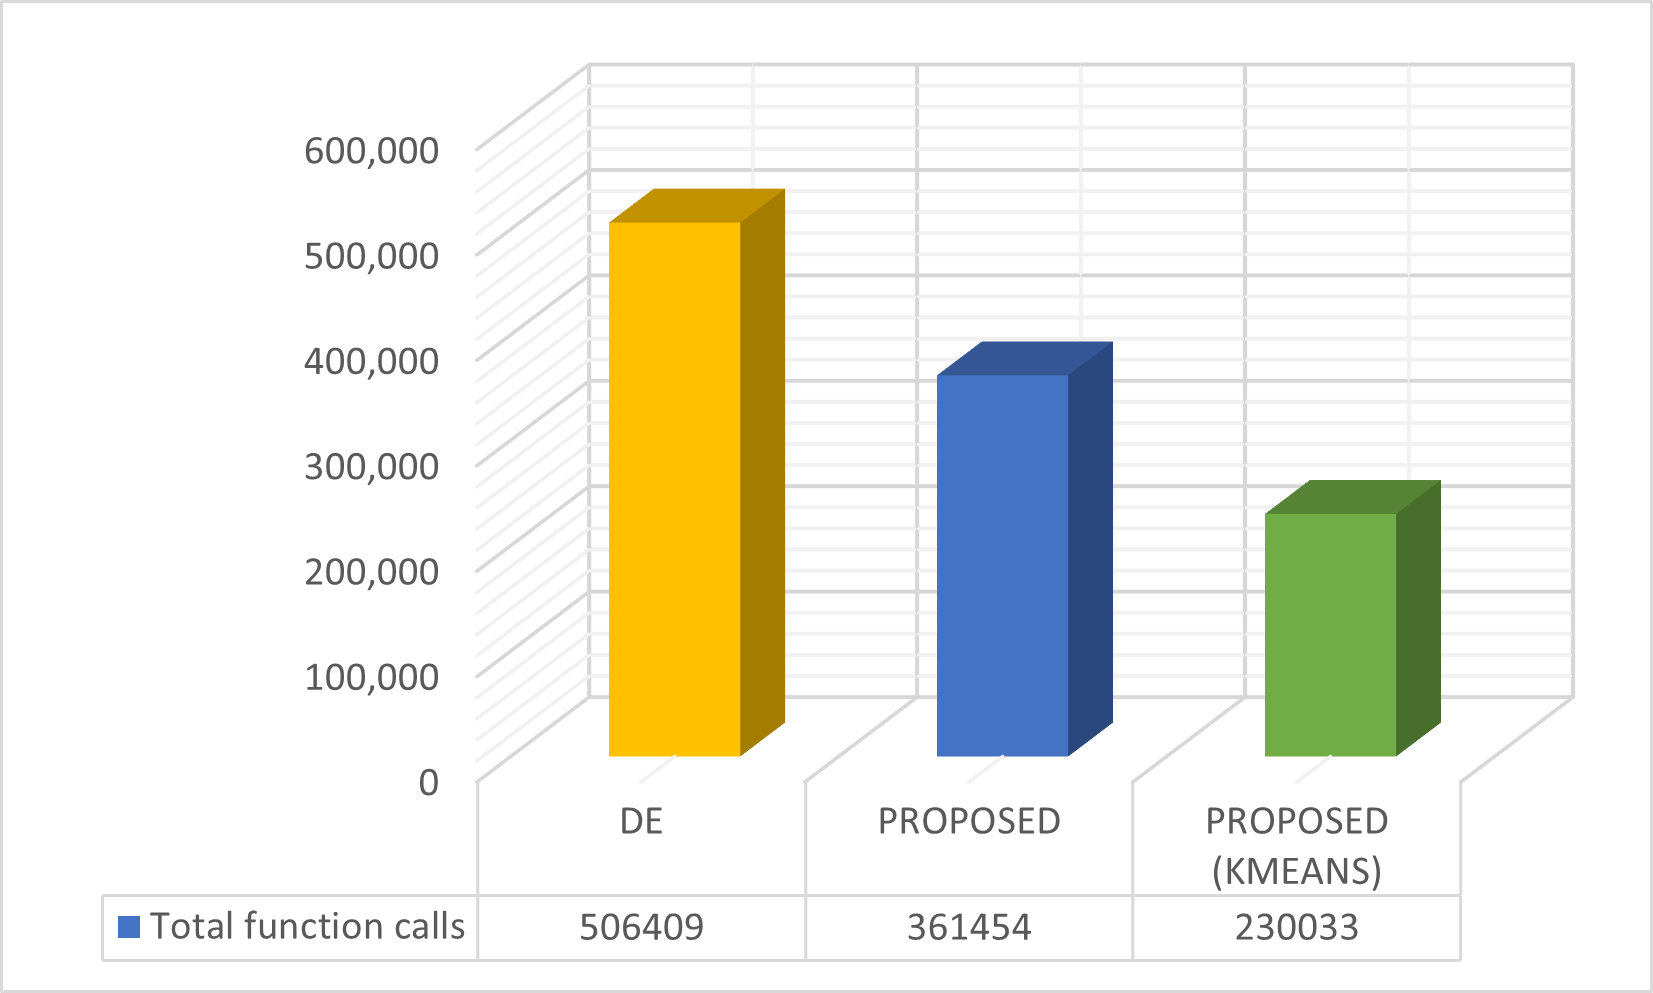
\includegraphics[scale=0.4]{new7}
\par\end{centering}
}\subfloat[Statistical comparison of total function calls\label{fig:compStatWithoutOutliers}]{
\centering{}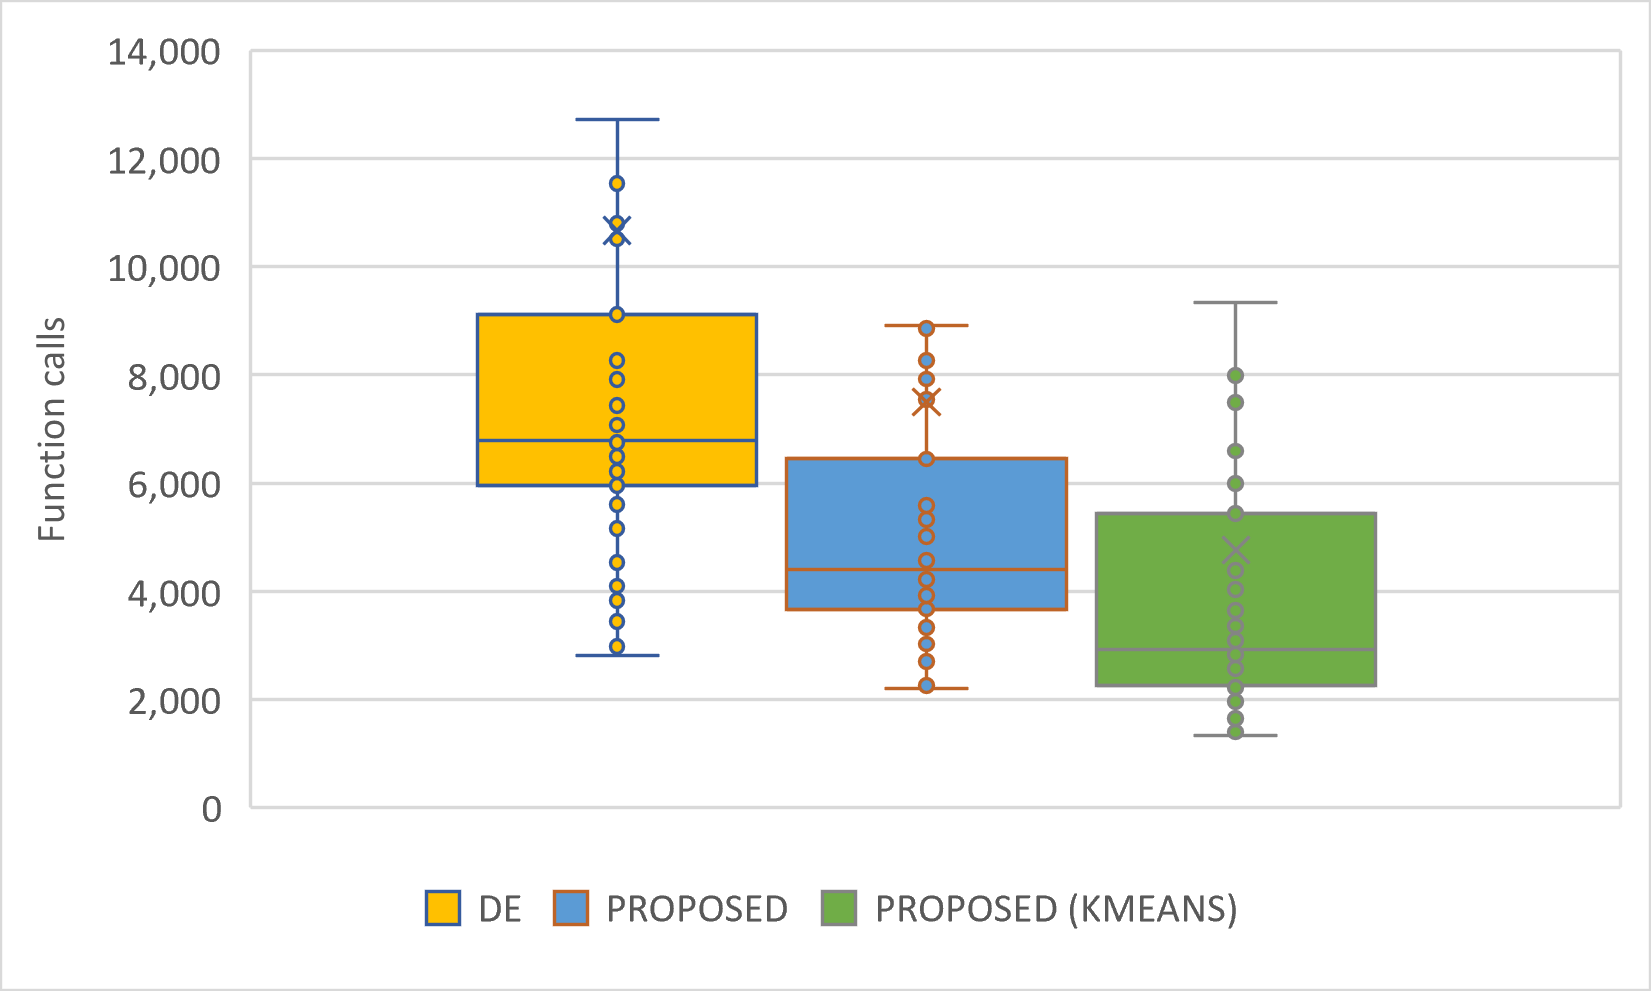
\includegraphics[scale=0.4]{new4}}\caption{Proposeds methods against DE\label{fig:proposedsVSDE}}
\end{figure}
\par\end{center}

\section{Conclusions\label{sec:Conclusions}}

An innovative global optimization method has been proposed in this
research paper, which leverages techniques derived from well-established
optimization strategies. More specifically, the new method incorporates
genetic operators from Genetic Algorithms alongside the Linear Search
method to generate candidate solutions for the given objective functions.
These candidate solutions are then combined to create new solutions
utilizing approaches inspired by the Differential Evolution method.
To validate the effectiveness of this new optimization approach, a
comprehensive series of experiments were conducted on various problems
sourced from the existing literature. Additionally, numerical comparisons
were made with recognized global optimization techniques to provide
a clear benchmark. The results indicate that the proposed optimization
method exhibits significantly superior performance when compared to
alternative methods, particularly in terms of the number of calls
made to the objective function. Fewer calls to the objective function
suggest better overall efficiency, highlighting the proposed method's
ability to achieve optimal solutions with fewer evaluations. This
efficiency is particularly critical in scenarios where each function
call is computationally expensive. Statistical analyses, including
both the t-test and the Kruskal-Wallis test, confirm that the observed
differences in the number of calls between the proposed method and
other methods are statistically significant, with a p-value of less
than 0.05. This finding not only underscores the reduced resource
consumption of the proposed method but also affirms that it delivers
reliable results with enhanced efficiency. In summary, the proposed
method stands out in terms of efficiency when compared to other optimization
techniques, significantly decreasing the number of objective function
calls and optimizing overall computational cost. Potential enhancements
to the algorithm could involve identifying specific samples that contribute
more effectively to the discovery of the optimal solution. Furthermore,
since this method represents a novel approach to optimization, exploring
alternative termination criteria or varying the initial sample distributions
could lead to even greater performance improvements. By refining these
aspects, the method could further bolster its efficiency and effectiveness
in solving complex optimization problems.

\vspace{6pt}


\authorcontributions{The conceptualization of the idea and the design of the methodology,
as well as the supervision of the technical aspects related to the
software, were undertaken by V.C., I.G.T., and G.K. The experiments
were conducted using various datasets, and the comparative results
were presented by V.C., G.K. and A.M.G. The statistical analysis was
carried out by V.C. The manuscript was prepared by G.K. and the other
authors. All authors have reviewed and approved the final published
version.}

\funding{No external funding was received for this research.}

\institutionalreview{Not applicable.}

\informedconsent{Not applicable. }

\institutionalreview{Not applicable.}

\acknowledgments{This research has been financed by the European Union: Next Generation
EU through the Program Greece 2.0 National Recovery and Resilience
Plan, under the call RESEARCH--CREATE--INNOVATE, project name “iCREW:
Intelligent small craft simulator for advanced crew training using
Virtual Reality techniques” (project code: TAEDK-06195).}

\conflictsofinterest{The authors declare no conflicts of interest.}

\conflictsofinterest{No conflicts of interest are declared by the authors.}

\appendixtitles{no}

\reftitle{References}
\begin{thebibliography}{999}
\bibitem{go_math1}\textbf{Carrizosa, E., Molero-Río, C., \& Romero
Morales, D. (2021). Mathematical optimization in classification and
regression trees. Top, 29(1), 5-33.}

\bibitem{go_math2}Cánovas, M. J., Kruger, A., Phu, H. X., \& Théra,
M. (2020). Marco A. López, a Pioneer of Continuous Optimization in
Spain. Vietnam Journal of Mathematics, 48, 211-219.

\bibitem{go_math3}\textbf{Legat, B., Dowson, O., Garcia, J. D., \&
Lubin, M. (2022). MathOptInterface: a data structure for mathematical
optimization problems. INFORMS Journal on Computing, 34(2), 672-689.}

\bibitem{go_physics1}Iuliano, E. (2017). Global optimization of benchmark
aerodynamic cases using physics-based surrogate models. Aerospace
Science and Technology, 67, 273-286.

\bibitem{go_physics2}\textbf{Su, H., Zhao, D., Heidari, A. A., Liu,
L., Zhang, X., Mafarja, M., \& Chen, H. (2023). RIME: A physics-based
optimization. Neurocomputing, 532, 183-214.}

\bibitem{go_physics3}\textbf{Stilck França, D., \& Garcia-Patron,
R. (2021). Limitations of optimization algorithms on noisy quantum
devices. Nature Physics, 17(11), 1221-1227.}

\bibitem{go_chem1}\textbf{Zhang, J., \& Glezakou, V. A. (2021). Global
optimization of chemical cluster structures: Methods, applications,
and challenges. International Journal of Quantum Chemistry, 121(7),
e26553.}

\bibitem{go_chem2}\textbf{Hu, Y., Zang, Z., Chen, D., Ma, X., Liang,
Y., You, W., ... \& Zhang, Z. (2022). Optimization and evaluation
of SO2 emissions based on WRF-Chem and 3DVAR data assimilation. Remote
Sensing, 14(1), 220.}

\bibitem{go_chem3}\textbf{Jeraal, M. I., Sung, S., \& Lapkin, A.
A. (2021). A Machine Learning‐Enabled Autonomous Flow Chemistry Platform
for Process Optimization of Multiple Reaction Metrics. Chemistry‐Methods,
1(1), 71-77.}

\bibitem{go_med1}\textbf{Nour, M., Cömert, Z., \& Polat, K. (2020).
A novel medical diagnosis model for COVID-19 infection detection based
on deep features and Bayesian optimization. Applied Soft Computing,
97, 106580.}

\bibitem{go_med2}\textbf{Kaur, P., \& Singh, R. K. (2023). A review
on optimization techniques for medical image analysis. Concurrency
and Computation: Practice and Experience, 35(1), e7443.}

\bibitem{medicine}Houssein, E. H., Hosney, M. E., Mohamed, W. M.,
Ali, A. A., \& Younis, E. M. (2023). Fuzzy-based hunger games search
algorithm for global optimization and feature selection using medical
data. Neural Computing and Applications, 35(7), 5251-5275.

\bibitem{go_bio1}\textbf{Wang, L., Cao, Q., Zhang, Z., Mirjalili,
S., \& Zhao, W. (2022). Artificial rabbits optimization: A new bio-inspired
meta-heuristic algorithm for solving engineering optimization problems.
Engineering Applications of Artificial Intelligence, 114, 105082.}

\bibitem{go_bio2}\textbf{Hesami, M., \& Jones, A. M. P. (2020). Application
of artificial intelligence models and optimization algorithms in plant
cell and tissue culture. Applied Microbiology and Biotechnology, 104(22),
9449-9485.}

\bibitem{go_agri1}Filip, M., Zoubek, T., Bumbalek, R., Cerny, P.,
Batista, C. E., Olsan, P., ... \& Findura, P. (2020). Advanced computational
methods for agriculture machinery movement optimization with applications
in sugarcane production. Agriculture, 10(10), 434.

\bibitem{go_agri2}\textbf{Akintuyi, O. B. (2024). Adaptive AI in
precision agriculture: a review: investigating the use of self-learning
algorithms in optimizing farm operations based on real-time data.
Research Journal of Multidisciplinary Studies, 7(02), 016-030.}

\bibitem{go_econ1}\textbf{Wang, Y., Ma, Y., Song, F., Ma, Y., Qi,
C., Huang, F., ... \& Zhang, F. (2020). Economic and efficient multi-objective
operation optimization of integrated energy system considering electro-thermal
demand response. Energy, 205, 118022.}

\bibitem{go_econ2}\textbf{Alirahmi, S. M., Mousavi, S. B., Razmi,
A. R., \& Ahmadi, P. (2021). A comprehensive techno-economic analysis
and multi-criteria optimization of a compressed air energy storage
(CAES) hybridized with solar and desalination units. Energy Conversion
and Management, 236, 114053.}

\bibitem{go_determ1}\textbf{Shezan, S. A., Ishraque, M. F., Shafiullah,
G. M., Kamwa, I., Paul, L. C., Muyeen, S. M., ... \& Kumar, P. P.
(2023). Optimization and control of solar-wind islanded hybrid microgrid
by using heuristic and deterministic optimization algorithms and fuzzy
logic controller. Energy reports, 10, 3272-3288.}

\bibitem{go_determ2}Cuevas-Velásquez, V., Sordo-Ward, A., García-Palacios,
J. H., Bianucci, P., \& Garrote, L. (2020). Probabilistic model for
real-time flood operation of a dam based on a deterministic optimization
model. Water, 12(11), 3206.

\bibitem{go_determ3}\textbf{Xu, Z., Zhao, Z., \& Liu, J. (2024).
Deterministic Multi-Objective Optimization of Analog Circuits. Electronics,
13(13), 2510.}

\bibitem{stohastic}\textbf{Hsieh, Y. P., Karimi Jaghargh, M. R.,
Krause, A., \& Mertikopoulos, P. (2024). Riemannian stochastic optimization
methods avoid strict saddle points. Advances in Neural Information
Processing Systems, 36.}

\bibitem{stohastic1}\textbf{Tyurin, A., \& Richtárik, P. (2024).
Optimal time complexities of parallel stochastic optimization methods
under a fixed computation model. Advances in Neural Information Processing
Systems, 36.}

\bibitem{stohastic2}Chen, T., Sun, Y., \& Yin, W. (2021). Solving
stochastic compositional optimization is nearly as easy as solving
stochastic optimization. IEEE Transactions on Signal Processing, 69,
4937-4948.

\bibitem{interval1}\textbf{Villanueva, F. R., \& de Oliveira, V.
A. (2022). Necessary optimality conditions for interval optimization
problems with functional and abstract constraints. Journal of Optimization
Theory and Applications, 194(3), 896-923.}

\bibitem{interval2}\textbf{Wang, L., Chen, Z., Yang, G., Sun, Q.,
\& Ge, J. (2020). An interval uncertain optimization method using
back-propagation neural network differentiation. Computer Methods
in Applied Mechanics and Engineering, 366, 113065.}

\bibitem{Sergeyev}Sergeyev, Y. D., Kvasov, D. E., \& Mukhametzhanov,
M. S. (2018). On the efficiency of nature-inspired metaheuristics
in expensive global optimization with limited budget. Scientific reports,
8(1), 453.

\bibitem{genetic1}\textbf{Chen, M., Yu, L., Zhi, C., Sun, R., Zhu,
S., Gao, Z., ... \& Zhang, Y. (2022). Improved faster R-CNN for fabric
defect detection based on Gabor filter with Genetic Algorithm optimization.
Computers in Industry, 134, 103551.}

\bibitem{genetic2}\textbf{Sohail, A. (2023). Genetic algorithms in
the fields of artificial intelligence and data sciences. Annals of
Data Science, 10(4), 1007-1018.}

\bibitem{genetic3}Charilogis, V., Tsoulos, I. G., \& Stavrou, V.
N. (2023). An Intelligent Technique for Initial Distribution of Genetic
Algorithms. Axioms, 12(10), 980.

\bibitem{diffe1}\textbf{Deng, W., Shang, S., Cai, X., Zhao, H., Song,
Y., \& Xu, J. (2021). An improved differential evolution algorithm
and its application in optimization problem. Soft Computing, 25, 5277-5298.}

\bibitem{diffe2}\textbf{Pant, M., Zaheer, H., Garcia-Hernandez, L.,
\& Abraham, A. (2020). Differential Evolution: A review of more than
two decades of research. Engineering Applications of Artificial Intelligence,
90, 103479.}

\bibitem{pso_major}\textbf{Shami, T. M., El-Saleh, A. A., Alswaitti,
M., Al-Tashi, Q., Summakieh, M. A., \& Mirjalili, S. (2022). Particle
swarm optimization: A comprehensive survey. Ieee Access, 10, 10031-10061.}

\bibitem{pso1}\textbf{Gad, A. G. (2022). Particle swarm optimization
algorithm and its applications: a systematic review. Archives of computational
methods in engineering, 29(5), 2531-2561.} 

\bibitem{pso2}\textbf{Shafiei Chafi, Z., \& Afrakhte, H. (2021).
Short‐Term Load Forecasting Using Neural Network and Particle Swarm
Optimization (PSO) Algorithm. Mathematical Problems in Engineering,
2021(1), 5598267.}

\bibitem{aco1}\textbf{Rokbani, N., Kumar, R., Abraham, A., Alimi,
A. M., Long, H. V., Priyadarshini, I., \& Son, L. H. (2021). Bi-heuristic
ant colony optimization-based approaches for traveling salesman problem.
Soft Computing, 25, 3775-3794.}

\bibitem{aco2}\textbf{Wu, L., Huang, X., Cui, J., Liu, C., \& Xiao,
W. (2023). Modified adaptive ant colony optimization algorithm and
its application for solving path planning of mobile robot. Expert
Systems with Applications, 215, 119410.}

\bibitem{fish}\textbf{Pourpanah, F., Wang, R., Lim, C. P., Wang,
X. Z., \& Yazdani, D. (2023). A review of artificial fish swarm algorithms:
Recent advances and applications. Artificial Intelligence Review,
56(3), 1867-1903.}

\bibitem{dolphin}\textbf{Kareem, S. W., Mohammed, A. S., \& Khoshabaa,
F. S. (2023). Novel nature-inspired meta-heuristic optimization algorithm
based on hybrid dolphin and sparrow optimization. International Journal
of Nonlinear Analysis and Applications, 14(1), 355-373.} 

\bibitem{WOA}\textbf{Nadimi-Shahraki, M. H., Zamani, H., Asghari
Varzaneh, Z., \& Mirjalili, S. (2023). A systematic review of the
whale optimization algorithm: theoretical foundation, improvements,
and hybridizations. Archives of Computational Methods in Engineering,
30(7), 4113-4159.}

\bibitem{WOA1}\textbf{Brodzicki, A., Piekarski, M., \& Jaworek-Korjakowska,
J. (2021). The whale optimization algorithm approach for deep neural
networks. Sensors, 21(23), 8003.}

\bibitem{WOA2}\textbf{Zan, J. (2022). Research on robot path perception
and optimization technology based on whale optimization algorithm.
Journal of Computational and Cognitive Engineering, 1(4), 201-208.}

\bibitem{key-7}\textbf{Lalwani, S., Sharma, H., Satapathy, S. C.,
Deep, K., \& Bansal, J. C. (2019). A survey on parallel particle swarm
optimization algorithms. Arabian Journal for Science and Engineering,
44, 2899-2923.}

\bibitem{key-8}\textbf{Harada, T., \& Alba, E. (2020). Parallel genetic
algorithms: a useful survey. ACM Computing Surveys (CSUR), 53(4),
1-39.}

\bibitem{gpu1}\textbf{Hussain, M. M., \& Fujimoto, N. (2020). GPU-based
parallel multi-objective particle swarm optimization for large swarms
and high dimensional problems. Parallel Computing, 92, 102589.}

\bibitem{gpu2}\textbf{Skinderowicz, R. (2020). Implementing a GPU-based
parallel MAX--MIN Ant System. Future Generation Computer Systems,
106, 277-295.}

\bibitem{gpu3}\textbf{Schmitz, A., Burak, S., Miller, J., \& Müller,
M. S. (2024). Parallel pattern compiler for automatic global optimizations.
Parallel Computing, 103112.}

\bibitem{holland}Holland, J. H. (1992). Genetic algorithms. Scientific
american, 267(1), 66-73.

\bibitem{ga_problem1}Hervis Santana, Y., Martinez Alonso, R., Guillen
Nieto, G., Martens, L., Joseph, W., \& Plets, D. (2022). Indoor genetic
algorithm-based 5G network planning using a machine learning model
for path loss estimation. Applied Sciences, 12(8), 3923.

\bibitem{ga_problem2}Liu, X., Jiang, D., Tao, B., Jiang, G., Sun,
Y., Kong, J., ... \& Chen, B. (2022). Genetic algorithm-based trajectory
optimization for digital twin robots. Frontiers in Bioengineering
and Biotechnology, 9, 793782.

\bibitem{ga_problem3}Nonoyama, K., Liu, Z., Fujiwara, T., Alam, M.
M., \& Nishi, T. (2022). Energy-efficient robot configuration and
motion planning using genetic algorithm and particle swarm optimization.
Energies, 15(6), 2074.

\bibitem{ga_problem4}Liu, K., Deng, B., Shen, Q., Yang, J., \& Li,
Y. (2022). Optimization based on genetic algorithms on energy conservation
potential of a high speed SI engine fueled with butanol--gasoline\LyXZeroWidthSpace{}
blends. Energy Reports, 8, 69-80.

\bibitem{ga_problem5}Zhou, G., Zhu, Z., \& Luo, S. (2022). Location
optimization of electric vehicle charging stations: Based on cost
model and genetic algorithm. Energy, 247, 123437.

\bibitem{ga_nn1}Arifovic, J., \& Gencay, R. (2001). Using genetic
algorithms to select architecture of a feedforward artificial neural
network. Physica A: Statistical mechanics and its applications, 289(3-4),
574-594.

\bibitem{ga_nn2}Leung, F. H. F., Lam, H. K., Ling, S. H., \& Tam,
P. K. S. (2003). Tuning of the structure and parameters of a neural
network using an improved genetic algorithm. IEEE Transactions on
Neural networks, 14(1), 79-88.

\bibitem{de_symmetry1}Li, Y. H., Wang, J. Q., Wang, X. J., Zhao,
Y. L., Lu, X. H., \& Liu, D. L. (2017). Community detection based
on differential evolution using social spider optimization. Symmetry,
9(9), 183.

\bibitem{de_symmetry2}Yang, W., Siriwardane, E. M. D., Dong, R.,
Li, Y., \& Hu, J. (2021). Crystal structure prediction of materials
with high symmetry using differential evolution. Journal of Physics:
Condensed Matter, 33(45), 455902.

\bibitem{de_problem1}Maulik, U., \& Saha, I. (2010). Automatic fuzzy
clustering using modified differential evolution for image classification.
IEEE transactions on Geoscience and Remote sensing, 48(9), 3503-3510.

\bibitem{de_problem2}Zhang, Y., Zhang, H., Cai, J., \& Yang, B. (2014).
A weighted voting classifier based on differential evolution. In Abstract
and applied analysis (Vol. 2014, No. 1, p. 376950). Hindawi Publishing
Corporation.

\bibitem{de_problem3}Hancer, E. (2019). Differential evolution for
feature selection: a fuzzy wrapper--filter approach. Soft Computing,
23, 5233-5248.

\bibitem{de_problem4}Vivekanandan, T., \& Iyengar, N. C. S. N. (2017).
Optimal feature selection using a modified differential evolution
algorithm and its effectiveness for prediction of heart disease. Computers
in biology and medicine, 90, 125-136.

\bibitem{de_deep1}Deng, W., Liu, H., Xu, J., Zhao, H., \& Song, Y.
(2020). An improved quantum-inspired differential evolution algorithm
for deep belief network. IEEE Transactions on Instrumentation and
Measurement, 69(10), 7319-7327.

\bibitem{de_deep2}Wu, T., Li, X., Zhou, D., Li, N., \& Shi, J. (2021).
Differential evolution based layer-wise weight pruning for compressing
deep neural networks. Sensors, 21(3), 880.

\bibitem{go_local2}Badem, H., Basturk, A., Caliskan, A., \& Yuksel,
M. E. (2018). A new hybrid optimization method combining artificial
bee colony and limited-memory BFGS algorithms for efficient numerical
optimization. Applied Soft Computing, 70, 826-844.

\bibitem{go_local3}Nagra, A. A., Han, F., \& Ling, Q. H. (2019).
An improved hybrid self-inertia weight adaptive particle swarm optimization
algorithm with local search. Engineering Optimization, 51(7), 1115-1132.

\bibitem{hybrid1}Li, S., Tan, M., Tsang, I. W., \& Kwok, J. T. Y.
(2011). A hybrid PSO-BFGS strategy for global optimization of multimodal
functions. IEEE Transactions on Systems, Man, and Cybernetics, Part
B (Cybernetics), 41(4), 1003-1014.

\bibitem{hybrid2}Andalib Sahnehsaraei, M., Mahmoodabadi, M. J., Taherkhorsandi,
M., Castillo-Villar, K. K., \& Mortazavi Yazdi, S. M. (2015). A hybrid
global optimization algorithm: particle swarm optimization in association
with a genetic algorithm. Complex System Modelling and Control Through
Intelligent Soft Computations, 45-86.

\bibitem{armijo}Armijo, L. (1966). Minimization of functions having
Lipschitz continuous first partial derivatives. Pacific Journal of
mathematics, 16(1), 1-3.

\bibitem{kmeansNew}Ahmed, M., Seraj, R., \& Islam, S. M. S. (2020).
The k-means algorithm: A comprehensive survey and performance evaluation.
Electronics, 9(8), 1295.

\bibitem[(2002)]{bfgs} Dai, Y. H. (2002). Convergence properties
of the BFGS algoritm. SIAM Journal on Optimization, 13(3), 693-701.

\bibitem{charilogis}Charilogis, V., \& Tsoulos, I. G. (2022). Toward
an ideal particle swarm optimizer for multidimensional functions.
Information, 13(5), 217.

\bibitem{Gaviano} Gaviano, M., Kvasov, D. E., Lera, D., \& Sergeyev,
Y. D. (2003). Algorithm 829: Software for generation of classes of
test functions with known local and global minima for global optimization.
ACM Transactions on Mathematical Software (TOMS), 29(4), 469-480.

\bibitem{Lennard} Jones, J. E. (1924). On the determination of molecular
fields.---II. From the equation of state of a gas. Proceedings of
the Royal Society of London. Series A, Containing Papers of a Mathematical
and Physical Character, 106(738), 463-477.

\bibitem{Zabinsky}Zabinsky, Z. B., Graesser, D. L., Tuttle, M. E.,
\& Kim, G. I. (1992). Global optimization of composite laminates using
improving hit and run. In Recent advances in global optimization (pp.
343-368).

\bibitem{Ali1}Ali, M. M., Khompatraporn, C., \& Zabinsky, Z. B. (2005).
A numerical evaluation of several stochastic algorithms on selected
continuous global optimization test problems. Journal of global optimization,
31, 635-672.

\bibitem{Floudas1}Floudas, C. A., Pardalos, P. M., Adjiman, C., Esposito,
W. R., Gümüs, Z. H., Harding, S. T., ... \& Schweiger, C. A. (2013).
Handbook of test problems in local and global optimization (Vol. 33).
Springer Science \& Business Media.

\bibitem{key-6}\textbf{Storn, R. (1996, June). On the usage of differential
evolution for function optimization. In Proceedings of North American
fuzzy information processing (pp. 519-523). Ieee.}

\bibitem{key-2}\textbf{Mirjalili, S., Mirjalili, S. M., \& Lewis,
A. (2014). Grey wolf optimizer. Advances in engineering software,
69, 46-61.}

\bibitem{key-1}\textbf{Shen, Y., Zhang, C., Gharehchopogh, F. S.,
\& Mirjalili, S. (2023). An improved whale optimization algorithm
based on multi-population evolution for global optimization and engineering
design problems. Expert Systems with Applications, 215, 119269.}

\bibitem{powell}Powell, M. J. D. (1989). A tolerant algorithm for
linearly constrained optimization calculations. Mathematical Programming,
45, 547-566.

\end{thebibliography}

\end{document}
